% Modelo de TCC do Bacharelado em Ciência da Computação da UNIFESP 
% Baseado no Modelo de Documentos Academicos do ABNTex2  

\documentclass[	12pt, Times, openright, twoside, a4paper, english, brasil]{abntex2}


\usepackage{cmap}				
\usepackage{times}
\usepackage[T1]{fontenc}			
\usepackage[utf8]{inputenc}		 
\usepackage{lastpage}			
\usepackage{indentfirst}			 
\usepackage{color}				
\usepackage[table]{xcolor}
\usepackage{graphicx}			
\usepackage[portuguese, ruled, linesnumbered]{algorithm2e} 
\usepackage{amssymb} 
\usepackage{glossaries}
\usepackage{float}
\usepackage{multicol,multirow}
\usepackage{adjustbox}
\usepackage[brazilian,hyperpageref]{backref}	 
\usepackage[alf]{abntex2cite}	
\usepackage{datatool} 
\usepackage[justification=centering]{caption}

\usepackage{lscape,pdflscape}
\usepackage{booktabs}
\usepackage{siunitx} 
%\usepackage{pgfplotstable} 
\usepackage{hyperref}
\hypersetup{colorlinks=False,  linkcolor=black,   filecolor=magenta, urlcolor=cyan }
\urlstyle{same}
\usepackage{listings}
\usepackage{booktabs}
\usepackage{stackengine}%
\usepackage{url}
\makeatletter
\g@addto@macro{\UrlBreaks}{\UrlOrds}
\makeatother

\usepackage{color}
\newcommand{\TODO}[1]{{\textcolor{red}{\textsf{TODO: #1}}}}
\newcommand{\TODOR}[1]{{\textcolor{blue}{\textsf{RESP: #1}}}}
\newcommand{\TEXTO}[1]{{\textcolor{magenta}{#1}}}


\definecolor{dkgreen}{rgb}{0,0.6,0}
\definecolor{gray}{rgb}{0.5,0.5,0.5}
\definecolor{mauve}{rgb}{0.58,0,0.82}
\lstset{
  language=Python,                
  basicstyle=\footnotesize,           
  numbers=left,                   
  numberstyle=\tiny\color{gray},  
  stepnumber=2,                             
  numbersep=5pt,                  
  backgroundcolor=\color{white},    
  showspaces=false,               
  showstringspaces=false,         
  showtabs=false,                 
  frame=single,                   
  rulecolor=\color{black},        
  tabsize=2,                      
  captionpos=b,                   
  breaklines=true,                
  breakatwhitespace=false,        
  title=\lstname,                               
  keywordstyle=\color{blue},          
  commentstyle=\color{dkgreen},       
  stringstyle=\color{mauve},     
}
% --- 
% CONFIGURAÇÕES DE PACOTES

\sisetup{  round-mode = places,  round-precision  = 2}

% ---
% Configurações do pacote backref
% Usado sem a opção hyperpageref de backref
  \renewcommand{\backrefpagesname}{Citado na(s) página(s):~}
%   Texto padrão antes do número das páginas
  \renewcommand{\backref}{}
%   Define os textos da citação
  \renewcommand*{\backrefalt}[4]{
  	\ifcase #1 	Nenhuma citação no texto.  	\or	Citado na página #2.%
  	\else Citado #1 vezes nas páginas #2.  	\fi}%
  % ---

  % numeração de figuras e elas 
  \counterwithout{figure}{section}
  \counterwithout{table}{section}

 \setlength{\parindent}{1.3cm}
 \setlength{\parskip}{\onelineskip}
 
   \makeatletter
  \hypersetup{
       	%pagebackref=true,
  		pdftitle={\@title}, 
  		pdfauthor={\@author},
      	pdfsubject={\imprimirpreambulo},
  	    pdfcreator={LaTeX with abnTeX2},
  		pdfkeywords={abnt}{latex}{abntex}{abntex2}{trabalho acadêmico},  colorlinks=false, linkcolor=blue, citecolor=blue,filecolor=magenta,  urlcolor=blue,
  		bookmarksdepth=4}

  \makeatother


  \makeindex


  \titulo{DEMAND ANALYSIS OF UNIVERSITY REFECTORY AT ICT UNIFESP VIA NEURAL NETWORKS.}
  \autor{Douglas Diniz Landim}
  \local{São José dos Campos, SP}
  \data{October 2020}
  \orientador{Prof. Dr. Marcos Gon\c{c}alves Quiles}
  \instituicao{Federal University of São Paulo -- UNIFESP
    \par
    Institute of Science and Technology
    \par
    Bachelor's Degree in Computer Science}
  \tipotrabalho{Trabalho de Graduação}
  \preambulo{Monograph presented to the Institute of Science and Technology – UNIFESP for obtaining of the title of bachelor's degree in Computer Science.}

\begin{document}
 
 \frenchspacing 

  % ----------------------------------------------------------
  % ELEMENTOS PRÉ-TEXTUAIS

  % \pretextual

    
  % ----------------------------------------------------------
  % Capa

    \begin{capa}
      \begin{center}
       
\includegraphics[width=.25\textwidth]{logo-unifesp.pdf}
        \vspace*{\fill}
        
        {\ABNTEXchapterfont\large\imprimirautor}
        \vspace*{\fill}
        
        {\ABNTEXchapterfont\bfseries\Large\imprimirtitulo}
        \vspace*{\fill}\vspace*{\fill}
        
       \imprimirlocal
       \end{center}
    \end{capa}


  % Folha de rosto
    \imprimirfolhaderosto*


  % Inserir folha de aprovação
    % \includepdf{folhadeaprovacao_final.pdf}
  %
    \begin{folhadeaprovacao}
      \begin{center}
        {\ABNTEXchapterfont\large\imprimirautor}

        \vspace*{\fill}\vspace*{\fill}
        {\ABNTEXchapterfont\bfseries\Large\imprimirtitulo}
        \vspace*{\fill}
        
        \hspace{.45\textwidth}
        \begin{minipage}{.5\textwidth}
            \imprimirpreambulo
        \end{minipage}%
        \vspace*{\fill}
       \end{center}
        
       Trabalho para apresentar em Outubro/2020:

       \assinatura{\textbf{\imprimirorientador} \\ Orientador} 
       \assinatura{\textbf{Professora} \\ Dra. Daniela Leal Musa}
       \assinatura{\textbf{Professora} \\ Dra. Regina Célia Coelho}

          
       \begin{center}
        \vspace*{0.5cm}
        {\large\imprimirlocal}
        \par
        {\large\imprimirdata}
        \vspace*{1cm}
      \end{center}
      
    \end{folhadeaprovacao}



  % ----------------------------------------------------------

  % Dedicatória

    \begin{dedicatoria}
       \vspace*{\fill}
       \centering
       \noindent
       \textit{ Este trabalho é dedicado aos meus pais que apoiaram e sacrificaram esforços para me manter ativo nessa jornada, a todos os professores que me somaram conhecimentos, oportunidades e esperanças indo além de suas rotinas e agendas em prol do ensino, e principalmente à todos que me motivaram me oferecendo desafios para que eu pudesse enfrentá-los superando meus próprios limites } \vspace*{\fill}
    \end{dedicatoria}

  % Agradecimentos

    \begin{agradecimentos}
        \paragraph{Minha Jornada}
            Minha jornada pela graduação foi marcada por muita persistência, dificuldades e fracassos. Agradeço primeiramente a Deus por me dar fé e alimentar minha persistência e esperança. Apesar de todo o conteúdo técnico das mais de 40 disciplinas do meu curso, o que mais me agregou aprendizado foi o ambiente desafiador desta universidade; que somado à muitas dificuldades pessoais, acidentes, contra-tempos de saúde, profissão e família; constituiu o conjunto perfeito de desafios que me transformou em uma pessoa forte e destemida para enfrentar as cobranças do mercado, mais convicto e perseverante a cada nova tentativa de conquistar meus objetivos. Agradeço à minha família por sempre me apoiar dando tudo de si, aos meus professores que me orientaram e me motivaram, nas reuniões e chats online até nos finais de semana, aos meus amigos universitários, e a todos os colegas e colaboradores que conheci durante a graduação na Unifesp.
            
            \paragraph{Em especial, agradeço:}
                
            À professora Daniela Musa por ser minha primeira coordenadora de curso e orientadora quando ingressei na Unifesp.
            
            Aos professores das disciplinas que formaram minha base de conhecimento da ciência da computação e que me deram grande preparo para as minhas atividades acadêmicas, profissionais e nos diversos processos seletivos que participei no mercado. Aos professores Reginaldo Kuroshu, Bruno Kimura, Àlvaro Fazenda, Regina Coelho, Arlindo Flavio, Antonio Chaves, Ana Luiza e Otavio Lemos.
            
            À professora Camila Bertini  que na disciplina de simulação de sistemas me motivou nos primeiros estudos no tema deste trabalho, com uma realização de correlação com reamostragem de consumo x temperatura em 2016.
            
            À professora Flavia Martins de estatística, que me orientou algumas vezes em sua sala sobre a introdução teórica de predições com redes neurais, sua tese de doutorado foi bem complementar e enriquecedora na fundamentação teórica deste trabalho.
            
            Aos professores Vinícius Veloso e Fabio Faria, por me apresentarem a disciplina de inteligencia artificial. E ao Vinícius Veloso por me orientar na primeira parte deste trabalho e em todo o desenvolvimento de fundamentação teórica da primeira parte.
            
            Ao professor Marcos Quiles por me orientar nesta segunda parte do trabalho, me apresentando desde o início o trabalho com python, tensorflow, scikit learning, sobre as orientações mais específicas do aprendizado da rede neural. Em me orientar nas métricas de avaliação dos modelos e sobre a toda a metodologia experimental, além das revisões no texto final.
            
            À equipe de Data Science e Machine Learning Engineering da empresa 2RP-NET, especialista em análise de fraudes, dados, e trabalhos com aprendizado de máquina em Big-data, da qual recentemente fui integrado em setembro/2020 graças ao aprendizado adquirido neste trabalho acadêmico. E por ter disponibilizado um período extenso da reunião de equipe durante o nosso expediente para discutirmos os resultados e métricas deste trabalho, equipe da qual é composta por profissionais mestres e doutores em data science e machine learning.
            
            À todos os outros professores, colegas, alunos e colaboradores do instituto de ciência e tecnologia da UNIFESP.
                
            À minha família por ter me apoiado nesse longo período na UNIFESP.

         \end{agradecimentos}
 
 
 
  % Epígrafe
  
    \begin{epigrafe}
        \vspace*{\fill}
    	\begin{flushright}
    		\textit{Mesmo desacreditado e ignorado por todos, não posso desistir, pois para mim, vencer é nunca desistir.\\
    		(Albert Einstein)}
    	\end{flushright}
    \end{epigrafe}
 
 
  % ----------------------------------------------------------
  % RESUMOS
 
  % resumo em português
    \begin{resumo}
         O presente trabalho tem como objetivo o estudo de métodos para a previsão de vendas do restaurante universitário da Unifesp para evitar super-projeção de demanda com consequência de desperdício de alimentos, ou subprojeção com consequência de docentes ou discentes sem refeições. Em uma investigação anterior, realizada como trabalho de disciplina, o autor empregou métodos estatísticos para a análise do comportamento de consumo de refeições. Neste trabalho, foram desenvolvidos modelos de aprendizado de máquina, mais especificamente, redes neurais perceptron de múltiplas camadas e redes \textit{gated recurrent units}, com métodos de análises de dados coletados, preparação e pré-processamento das informações, seleção e avaliação dos melhores modelos e conclusões finais.
     
     \vspace{\onelineskip}
        
     \noindent
     \textbf{Palavras-chave}: Redes Neurais Artificiais, Previsão de demanda, Aprendizado de Máquina, Inteligência Artificial, Perceptron Múltiplas camadas. 
     
    \end{resumo}

  % resumo em inglês
    \begin{resumo}[Abstract]
     \begin{otherlanguage*}{english}

% TRADUZIR NOVAMENTE DO RESUMO ALTERADO

        This current work aims to study methods for forecasting meals of Unifesp university restaurant to avoid over-projection of demand resulting from food waste, or under projection with the consequence of teachers or students without meals. In a previous investigation, carried out as discipline work, the author used statistical methods to analyze meal consumption behavior. Machine learning models were developed in this work, more specifically, multilayer perceptron neural networks and gated recurrent units networks, with data analysis methods, preparation and pre-processing of information, selection, and evaluation of the best models and final conclusions.

       \vspace{\onelineskip}
     
       \noindent 
       \textbf{Keywords}: Artificial Neural Networks, Demand Prediction, Machine Learning, Artificial intelligence, Perceptron Multiple layers.
     \end{otherlanguage*}
    \end{resumo}


  % ----------------------------------------------------------
  
  % Lista de ilustrações
    \pdfbookmark[0]{\listfigurename}{lof}
    \listoffigures*
    \cleardoublepage

  % Lista de tabelas
    \pdfbookmark[0]{\listtablename}{lot}
    \listoftables*
    \cleardoublepage


  % ---  % Lsta de abreviaturas e siglas
  % ---
    \begin{siglas}
    \item[ICT] Instituto de Ciência e Tecnologia
    \item[R.U.] Restaurante Universitário
    \item[UNIFESP] Universidade Federal de São Paulo
    \item[UFV] Universidade Federal de Viçosa
    \item[UNESP] Universidade Estadual Paulista Júlio de Mesquita Filho
    \item[BDMEP] Banco de Dados Meteorológicos para Ensino e Pesquisa
    \item[RNA] Rede Neural Artificial
    \item[MLP] Multi Layer Perceptron
    \item[GRU] Gated Recurrent Unit
    \item[RMSE] Root Mean Squared Error

    \end{siglas}
 
  % ---
    \pdfbookmark[0]{\contentsname}{toc}
    \tableofcontents*
    \cleardoublepage
  % ---



  % ----------------------------------------------------------
  % ELEMENTOS TEXTUAIS
  % ----------------------------------------------------------
  \textual

  % ----------------------------------------------------------
  % CAPÍTULO 1 - Introdução
  % ----------------------------------------------------------
  
    \chapter{Introduction}

% \section{Contextualização e Motivação}

\noindent

Among the most accepted definitions of food security is the version coined during the 1996 World Food Summit \cite{shaw2007world}, which enunciates it as a situation where all people, at all times, have physical, social and economic conditions to access safe, healthy and nutritious food for a healthy and active life. However, according to the World Health Organization \cite{world2009global} over 1 billion people in the world have a nutritionally insufficient diet and more than twice as many people necessitate micronutrients.

According \citeonline{webb2006}food security can be decompose into 3 essential pillars, availability, possibility of access and rational utilization. These concepts are intrinsically
hierarchical since the availability does not guarantee access, which in turn does not guarantee its rational use. With the advances in agricultural production and the opening of world economic markets, although it has not solved the problem, it has made possible strides in the first two pillars of food security above-mentioned. Thus, in the first decades of the 21st century, the third pillar of the rational use of resources, has proved to be an important factor to be considered in this new globalized world. \cite{barrett2010}.

At the end of 2019, a highly communicable disease was identified in China's Wuhan province, commonly called the new Coronavirus (COVID-19), which was declared in a pandemic state in March 2020, and has so far infected more than 40 million people and caused 1 million  deaths.\footnote{\url{https://www.worldometers.info/coronavirus/}}. Despite global efforts to contain and remedy the COVID-19 pandemic, there are no scientifically proven vaccines or cures and the need for \textit{lockdown} is still pertinent to avoid new waves of contamination. The effects of the pandemic have been devastating in virtually all economic areas, especially in the food sector which is essential for maintaining life and has no room for \textit{lockdown} \cite{galanakis2020food}.

On 22 July 2020, the Brazilian Association of Food Industry and Consumption, held a conference on the impacts of the COVID-19 pandemic on the Brazilian food production chain\footnote{\url{{https://www.abia.org.br/noticias/abia-participa-de-live-para-discutir-os-impactos-da-pandemia-na-cadeia-produtiva-de-alimentos}}}. In this conference were brought together experts and executives from the agro-industrial sector to analyze changes in consumption behavior in the tertiary sectors that deal directly with the supply of food to the final consumer. From this analysis of the new consumer routine, new forecasting methods are being looked for the current format of consumption and the new demand for these sectors. Finally, methods of production and supply of agribusiness for the tertiary sector were also discussed.

Thus, in this chaotic period, when the global labor has reduced approximately 25\% during the first months of the pandemic
 \cite{huff2015resilient}, comes up the importance of developing processes that use food resources in the most rational way possible. Neste contexto, uma área que chama a atenção é a de previsão de demandas indústrias or from establishments that deal with perishable food in large quantities, since the food has an expiration date and production on demand can avoid storage for long periods or unwanted disposal of ready-to-eat foods.

In this sense, forecasting demands for meals in industrial or large restaurants, such as university refectory (RU) becomes viable, which meals are offered at affordable prices to the student community of the institution, through subsidies in the amount passed on to students. Generally, (RUs) are outsourced through bids in which the state government provides a percentage of each meal produced for the refectory management company. Due to health regulations, meals prepared but not consumed until the end of the working day should be discarded to avoid contamination and ensure the food safety of the consumer\footnote{\url{https://super.abril.com.br/mundo-estranho/o-que-acontece-com-a-comida-que-sobra-dos-restaurantes/}}. In this way, the excess production (not consumed) of meals by the (RU's) generates not only an exaggerated expenditure of public financial resources but also anunreasonable use of food resources.

In this context, Unifesp's university refectory in São José dos Campos is a good case study since it sells approximately 90 thousand meals annually, in which each meal has a fixed value of R\$2,50 for students and an subsidy of approximately R\$9,00 
per meal in the last decade (2011-2019). With this, more than 6 million reais were subsidized during the years 2011 to 2019.

One way to reduce this waste is in the development of consumption prediction methods \cite{Lopes2008,Rocha2011}.Usually, the approaches for forecasting the consumption demand of a university restaurant are summarized in the exploratory analysis of collected data, for example the sales computed in the previous week or month.  In addition, external information, denominated exogenous data, can be also considered in the prediction process, such as climate data, annual calendar data, holidays, among other information that may be relevant for consumption estimation.

The prediction of consumption of university refectory chains has already been discussed in earlier works.For example, in the work of \citeonline{Lopes2008} held at the UFV, a model of a perceptron neural network with 1 hidden layer and 1 output neuron is used, using the previous 5 days as prediction parameters with 3\% error over the total consumed, and in the work of \citeonline{Rocha2011} performed at UNESP is also used a neural network model with 1 hidden layer and 1 exit neuron, using only 1 parameter that informs the number of meals of the previous day, and other parameters informing averages of previous days and information regarding the date of consumption, this model obtained an error of 9,5\% calculated on the total consumed.

So, this work consists in the application of Neural Network models to forecast the demand for the meals provided at the university refectory of Unifesp in the campus of São José dos Campos. For this, it will be used a set of historical data available in the Unifesp system and other external (exogenous) information that can impact the consumption behavior and its prediction process.

The general objectives of this work include the construction and comparison of Artificial Neural Networks models for forecasting the demand for meals at the ICT-UNIFESP university refectory. Specifically, it has as objectives:
\begin{enumerate}[label=\alph*)]
\item Obtain and preprocess data of consumption and sale of meals from the refectory environment and data from the external environment to consumption, such as climate data, aiming their use as input of machine learning models to obtain the consumption predictions at the output of these models;
\item Execute exploratory and descriptive analysis of all data;
\item Build and evaluate predictive models of Neural Networks;
\item Execute analysis on the metrics of predictions of the models pointing their viable characteristics for a consumption prediction.
\end{enumerate}

The rest of this document is organized as following. The chapter \ref{cap:teoria} introduces the necessary foundation for the understanding of this work; The literature related to the subject is described in chapter \ref{cap:literatura}; The chapter \ref{cap:metodos} introduces the methodology used in this study; The results are summarized in chapter \ref{cap:resultados}; The main conclusions of this project as well as indications of future investigations are presented in chapter \ref{cap:conclusoes}; Lastly, chapter \ref{cap:anexo1} presents some additional results generated during the experiments and the implemented codes.

    \chapter{Theoretical Foundations } \label{cap:teoria}
  
In this chapter a quick review of the main characteristics of time series, as well as of Neural Networks, especially those that will be applied to the problem of interest, called Multilayer Perceptron Networks (MLP) and Gated Recurrent Unit (GRU).  

    \section{Demand Forecasting Methods} 
    
Demand forecasting can be defined as a process of searching for information that produces sales of a product or a set of products.

        In \citeonline{moreira1998} are defined as methods of demand forecasting that use such information to estimate future demand, and can fit this definition from subjective and intuitive methods to mathematical and computational methods. In the same article, the forecast models are classified into two major groups: qualitative methods and quantitative methods.
        
         In  \citeonline{Junior2007} has been made the evaluation of several methods of demand forecasting, which are schematized in the Figure  \ref{fig: metodosPrevisaoDemanda}. 
        
                  \begin{figure}[ht]
                  	\center{
                  	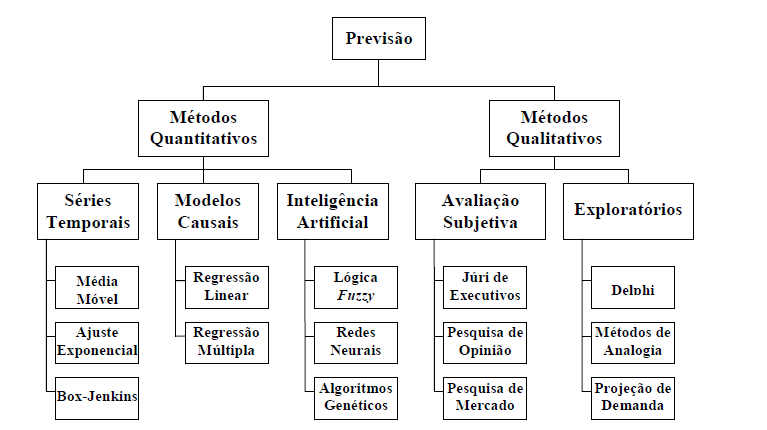
\includegraphics[width=\textwidth]{./Figs/01-junior-metodos-previsao-demanda.png}
                  	\caption{Demand forecasting methods.}\caption*{  Source: \cite{Junior2007}.}
                  	\label{fig: metodosPrevisaoDemanda}}
                  \end{figure}
        
        Quality methods are defined in \cite{Junior2007} as a judgment of the data exposed without processing analytics, such as grouping and classification of data. These methods do not provide new numerical information or predict models.
        
        On the other hand, quantitative methods are defined, in the same study, as being analytical and based on mathematical models for performing predictions. These methods analyze behavior patterns from a data historical, aiming to predict future behavior.
         
        In \citeonline{Junior2007} is also mentioned that the data collected for forecasting models, when graphically projected, show behaviors that can be generalized in a subjective way by managers of the data. For all cases, data analysis is necessary to select the parameters of the demand to make objective predictions.  Yet, only data analysis may be insufficient, and if performed with incorrect criteria it may compromise the conclusions of the studies. 
        
         Data analysis is a large process that aims to treat data from its acquisition and pre-processing until its interpretation using complex mining tools. In different steps, diverse mathematical, probabilistic, statistical, computational and heuristic techniques are involved.  In Section \ref{sec: timeseries} will be commented the main characteristics of the time series, which will be the forecasting method applied to the practical problem of interest. 
    
        \subsection{Time Series} \label{sec: timeseries} 
         
            According to \citeonline{Morettin1987}, a temporal series is a set of observations ordered in function of time, commonly the same, presenting a serial dependence among itself. Also it can be defined as a realization of a set of random variables  $ X=\{x_1, x_2, \dots, x_T\}$, ordered in time, where  $T$ represents the length of the series, as is made in \cite{defts}. The correlation between the variables is usually described by their collective distribution function or in other cases by the media and covariances. 
            
            Among the objectives of time series analysis, the following can be emphasized: i) describe the behavior of the series identifying trends and variations, ii) analyze and mold the dependency between the observations, and iii) fmake forecasts of future series values. 
            
            Time series have a deterministic component and a random component, they can be continuous or discrete, depending on the type of observation of the variables. They are called stationary when the properties of mean, variance and covariance are kept in time. The trend references the rate of growth or decrease, and can be linear, exponential or cushioned. Yet the oscillation of the trend is known as the cycle. In addition, they can present seasonality, in other words, exhibit behavior that has a tendency to repeat itself in a certain number of time periods.
    
             Examples of each of these properties, as well as techniques applied to study and correct each of them can be seen in \cite{tecnicas1}. These features, together with the random component study, provide information of interest for practical applications.
             
            %\TODOR{Passar pra metodologia ou literatura, não falar do trabalho aqui}
            Because of the objective of this work, temporal series will be applied for events with seasonality in order to estimate forecasts. The techniques to do this are using regression methods and some practical applications can be seen to include forecasting of realized power consumption, as made in \citeonline{Almeida2013}, \citeonline{RUAS2012} and \citeonline{Silva2010}, and of the demand forecast of cosmetic products, as it can be seen on\citeonline{Junior2007}.
    
    \section{Artificial Neural Networks}
    
        Artificial Neural Networks are tools with multidisciplinary basis, once they are nourished by knowledge of neuroscience, mathematics, statistics, physics, computer science and engineering \cite{Haykin1994}, and are part of the great area of knowledge called Artificial Intelligence (AI), term pointed out in \cite{kaplan2019siri}.
        
        In a nutshell, it could be defined that "artificial intelligence is the branch of computer science that deals with intelligent behavior. \cite{Luger2004}. Artificial Intelligence systems seek to solve functions and problems inspired by two human characteristics: the capacity for abstraction and learning from the error.
        
        In the context of Artificial Intelligence, a neuron is a unit considered fundamental for information processing, and Neural Networks are sets of artificial neurons interconnected through connections, logical and mathematical functions \cite{Haykin1994}. Neurons of a network are capable of processing multiple values of inputs and react quickly producing a related response to these inputs, simulating the behavior of the human brain. 
        
        Inspired by a search for a computational model of the biological neuron, the first artificial neuron model, called MCP, was proposed in the article \textit{ A Logical Calculus of the Ideas Immanent in Nervous Activity.} \cite{mcculloch43a}, an illustration adapted for \cite{lemos} of this model can be found in the figure \ref{fig: NeuronioArtificial}.
        
        McCuloch was a psychiatrist and neuroanatomist and spent about 20 years reflecting and studying about the representation of the nervous system, in 1942 he invited Pitts who was a mathematician to be part of his researches.
        
        The structure of the artificial neuron reacts to an input vector and synapses are represented by numerical weights. A transfer function also called the activation function, measures a linear combination of the input values and the synapses weights, determining if or not the neuron is activated depending on the value obtained. If the neuron is activated an output value of 1 is emitted, otherwise an output value of 0 is emitted.
            \begin{figure}[ht]
                \center{
                  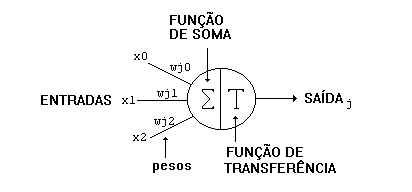
\includegraphics[width=0.65\textwidth]
                  {./Figs/02-neuronio-artificial.png}
                \caption{Artificial Neuron. }\caption*{  Source: \cite{lemos}} \label{fig: NeuronioArtificial} }
            \end{figure}
            
        The whole functionality of this model is then reduced to reply if the weighted sum received is greater than an established numerical value. Although, associated to this neuron was not proposed an automatic way to adjust the weights, that means no learning algorithm was given to train the neuron. This problem was later solved by Perceptron's formulation.
        
        In \citeonline{Haykin1994} in Chapter 1.9 entitled \textit{Historical Notes}, is introduced in more detail the fascinating history of the development of Neural Networks from the initial conception of biological neuron studies until complex networks of supervised learning known as \textit{Vector Support Machines}.
            
        \subsection{Perceptron} \label{sec: perceptron}
    
            The proposed neuron model in \citeonline{mcculloch43a}, even though it simulated a biological neuron and solved some logical and mathematical tasks, it did not satisfy the main objective of Artificial Intelligence: The capacity of learning. To be able to use this structure, it was necessary to know how to adjust the weights of the inputs, which was not a trivial problem in many cases. 
                        
            The first neuron with a learning algorithm was suggested in \citeonline{perceptron} and was named Perceptron. In this study, the weights of the connections are adjusted autonomously with the introduction of associated weights and a Bias value, in order to search for an autonomous recognition of standards. In the figure \ref{fig: perceptron} a schematic of the operation of the structure is presented.
            
            \begin{figure}[ht]
            	\center{
              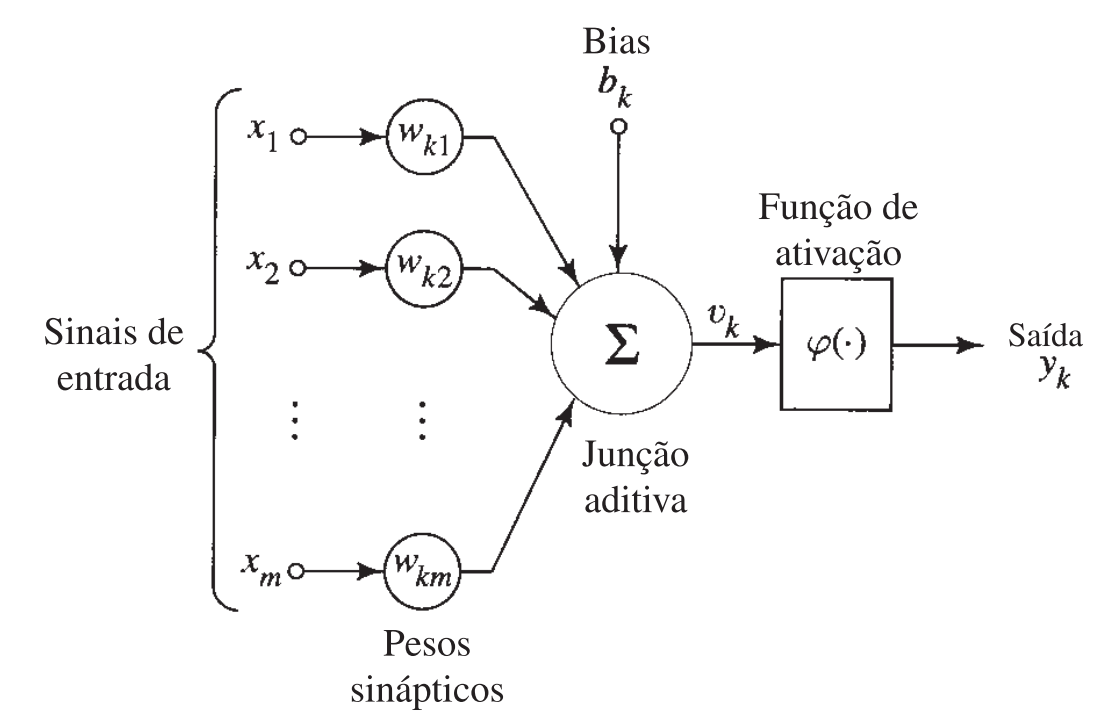
\includegraphics[width=0.65\textwidth]
              {./Figs/03-perceptron.png}
            \caption{Artificial Neuron Perceptron. }\caption*{  Source: \citeonline{Haykin1994}} \label{fig: perceptron} }
            \end{figure}
            
            But in \citeonline{perceptrons2} was proven that because of the learning model limited to a linear combination, the perceptron could only solve linearly separable problems. In the figure \ref{fig:problemasLineares} two simple problems are presented, one that perceptron can solve \textit{(a)}, and another does not \textit{(b)}.
            
            \begin{figure}[ht]
              	\center{
              	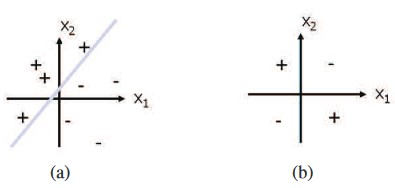
\includegraphics[width=0.8\textwidth]{./Figs/04-limite-perceptron.jpg}
              	\caption{Problem linearly separable (a) and not separable (b).}\caption*{  Source: \cite{Flavia2014}.}
              	\label{fig:problemasLineares}
              	}	
            \end{figure}
            
            Almost two decades later, it was released in \cite{rede1} the first model of a Neural Net, called a perceptron net, applying the training by linear combinations to a set of interconnected perceptrons. This approach allowed solving more complex problems through a combination of solutions. 
              
            The network had just one input layer, one output and an activation function  $ \varphi $ \cite{Haykin1994}. Perceptron network activation function could still be linear or non-linear. In the figure \ref{fig:activation_functions} some commonly used activation functions are illustrated. 
            
             \begin{figure}[ht]
                \center{
            	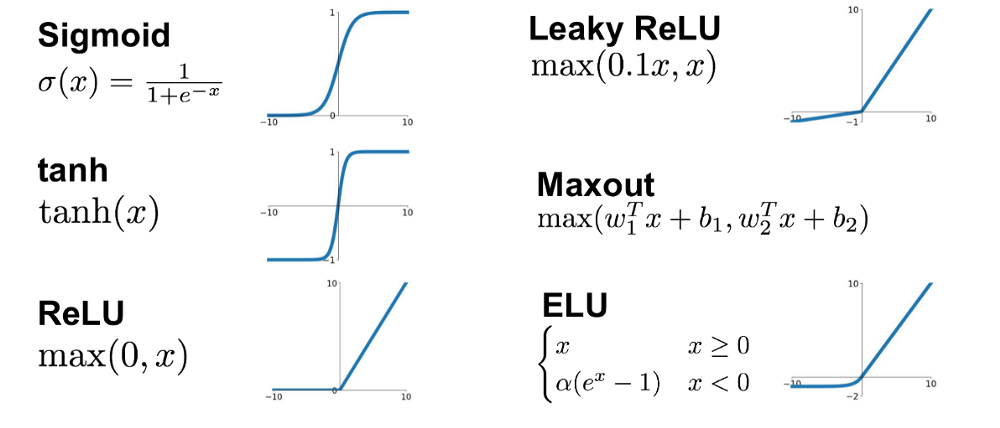
\includegraphics[width=0.80\textwidth] {./Figs/05-funcoes-ativacao.png}
                \caption{Examples of Activation functions.}\caption*{  Source: \cite{MCAI}} \label{fig:activation_functions}} 
            \end{figure}
            
            In \citeonline{Almeida2013} the learning process of the perceptron network is analyzed in a supervised way. During this process, the structure learns to relate an observed set of input variables in the network to one or more expected output values named as real values or truth values. Then the learning results are analyzed by comparing these values with the values generated by the perceptron net over the same set of data, and from this comparison is calculated the error measurement of the training.
                        
            A criterion for stopping training algorithm is to check whether the error is acceptable or not. If positive, the neural network maintains the values of the synapses weights obtained at the time. If not, a new training season is made trying to adjust the weights to obtain a smaller failure.
            The other criterion for stopping training is to reach a maximum number of training periods allowed. The adjustment of weights is called the rate of learning.
            
            The next step in developing Neural Network models is related to the topology that determines the amount of perceptrons in the network and how they connect, generating multi-layered networks.        
    
        \subsection{MultiLayer Network Perceptron (MLP)}
    
            The possibility of combining two or more layers of perceptrons was given by the use of an output signal combiner perceptron. With it the Neural Networks are scaled up to several interconnected perceptrons columns. Each column is denominated a hidden layer of the Neural Network. The last layer must have the number of perceptrons corresponding to the number of desired outputs. In the figure \ref{fig:MLP} a Neural Network with 2 hidden layers is presented, whose output layer has 3 neurons.
            
            \begin{figure}[ht]
             \center{
             	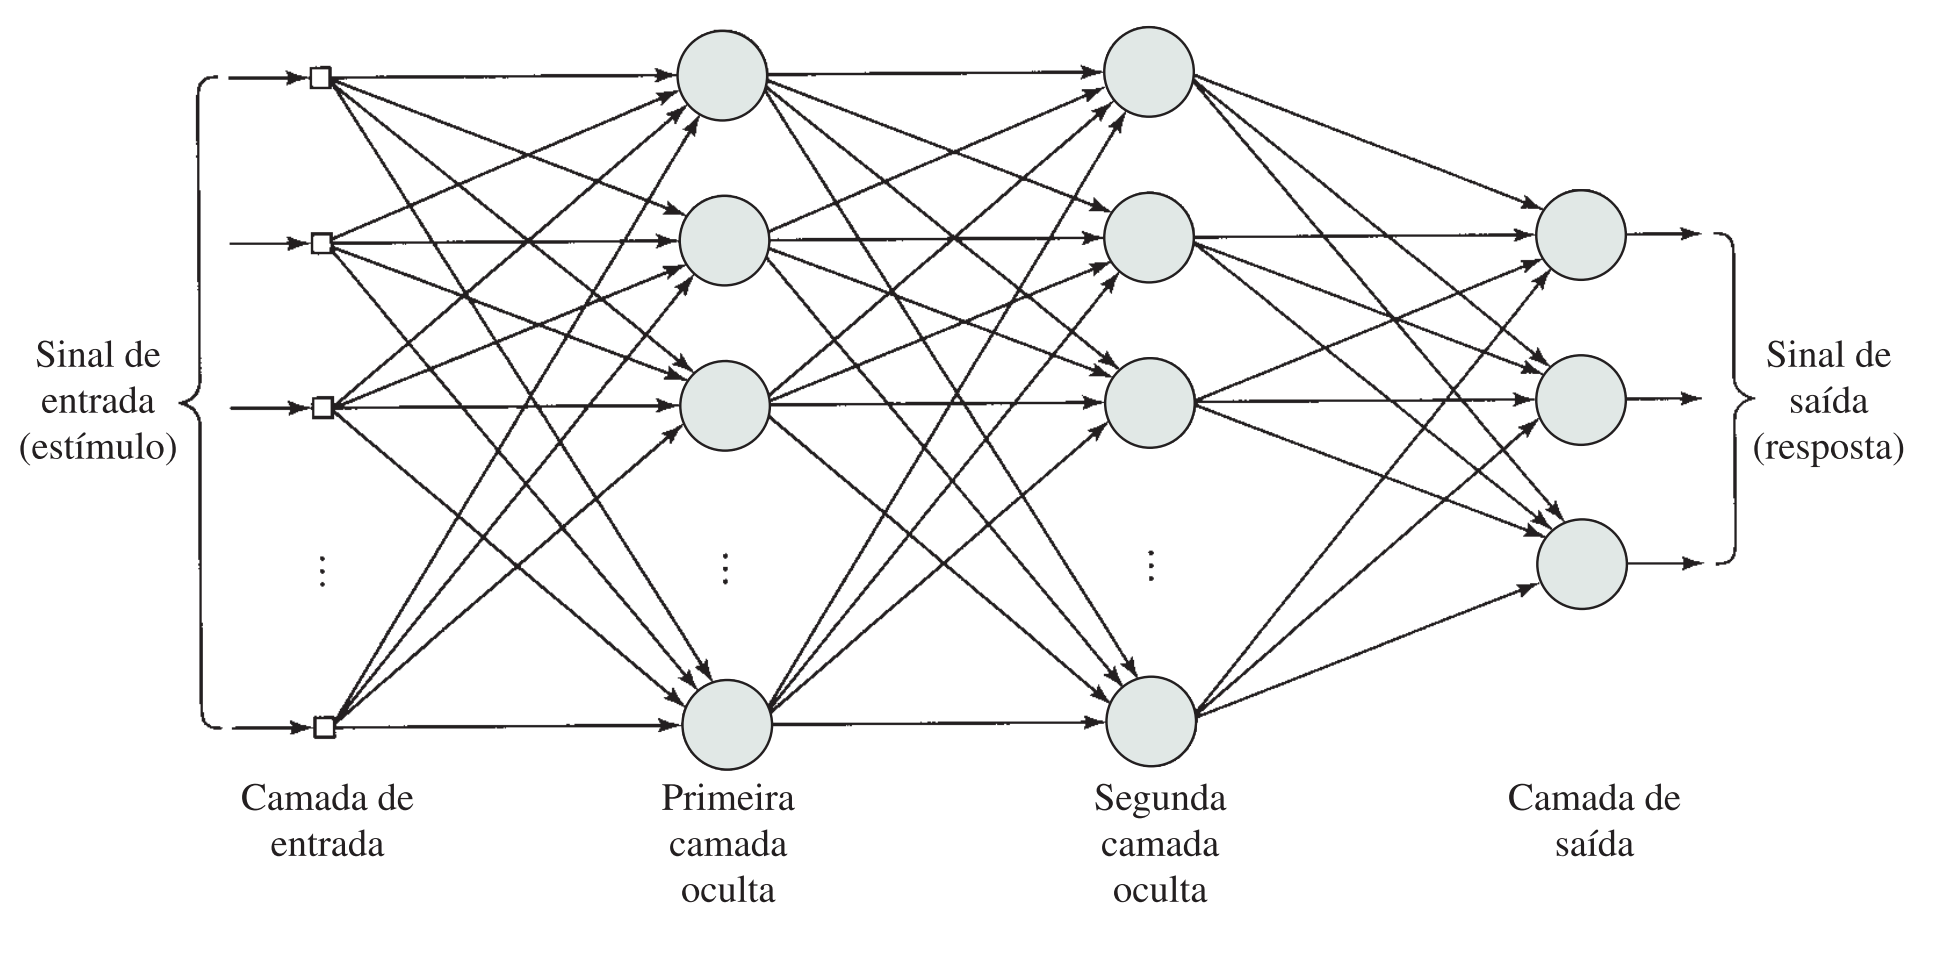
\includegraphics[width=\textwidth]
             	{./Figs/06-MLP.PNG}
             \caption{MultiLayer Network Perceptron. }\caption*{  Source: \cite{Haykin1994}\label{fig:MLP}
             }}
            \end{figure}
            
            In \citeonline{Braga2000} is postulated that through an intermediate layer it is possible to approximate any continuous function and further that two intermediate layers are enough to approximate any mathematical function. If the use of two or more layers can facilitate the training of the network, it becomes unviable to use a large number of these, since in each hidden layer the error is estimated from the error in the previous layer, which generates loss of accuracy.
            
            In practical applications, it has been seen that in some cases, the capacity for abstraction and recognition of Neural Network patterns overcome human capabilities. In other cases a network may not produce an expected response by incorrectly solving a problem, as well as the human brain, because of learning limitations or training failures. 
              
            To train an MLP network in a supervised way, the input data set must be divided into two subsets, one of \textit{training} and another of \textit{validation}. These subsets can be separated with various techniques. Thus, for example in \citeonline{DLB} a heuristic form of set separation in random order is presented, with 70\% of the data for training and 30\% of the data for validation.
            
            About the maximum number of training attempts allowed, very long training sessions tend to memorize weights of the values observed in the training data.  This implies a loss of network generalization capacity, resulting in a difficulty to evaluate entries outside the training data. This phenomenon is known as \textit{overfitting}.
            
            There is also another way of training an MLP network, called cross-validation, which was presented in \cite{crossvalidation}. This technique consists of exchanging the sets of training and validation at different times of training. In that case, the measurement of the validation error goes through an evaluation process taking into consideration the number of periods. By evaluating the average quadratic error of both sets it is possible to detect the beginning of the \textit{overfitting}. For this reason, the optimal stopping point of the training is associated with the lower limit of this mean square error in the validation set illustrated in the figure \ref{fig:validacaoCruzada} as an early stopping point for \textit{overfitting}.
            
            \begin{figure}[ht]
              \center{
              	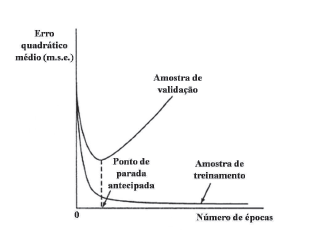
\includegraphics[width=0.5\textwidth]
              	{./Figs/07-validacaocruzada.png}
              
              \caption{Ideal stop point of cross validation. }\caption*{ Source: \cite{Haykin1994}} \label{fig:validacaoCruzada}} 
            \end{figure}
    
        \subsection{Multiple Layer Perceptron Network with \textit{Backpropagation}.}
    
            The learning method for multi-layered Neural Networks known as \textit{Backpropagation} was presented in \cite{backp}, as an abbreviation of \textit{backward propagation of errors}, in Portuguese, retro-propagação de erros. In this method, the training is conducted in two phases:
        
            \paragraph*{\textit{ Feed-forward} } An input vector with known output vector is presented to the neurons of the first layer, and an output vector is calculated according to the natural flow of operations in the network.
             
            \paragraph*{\textit{Feed-backward}} The error gradient is calculated to obtain information that induces a decrease in function, given by the opposite direction to the gradient. With this, the weights of all layers are updated, starting with the last one and following the inverse flow of the network.
             
            These two phases are schematized in Figure \ref{fig: MLP2}. 
             
            \begin{figure}[ht]
             	\center{
             		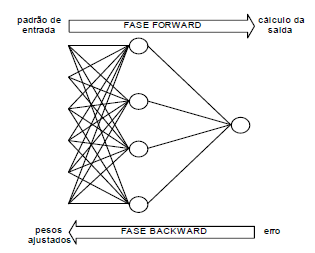
\includegraphics[width=0.65\textwidth]
             		{./Figs/08-mlp-back.png}
             	
             	\caption{Training phases of the MLP-Back-Propagation}.}\caption*{  Source:  \cite{Almeida2013}}\label{fig: MLP2}}
            \end{figure}
            
            In this method, as the error gradient is calculated from the lower to the upper layers, its norm decreases with exponential speed. This makes that in the layers closest to the entrance the weight adjustments are small, making the learning in them slower. This problem is known in the literature as \textit{vanishing gradient problem}. Usually the values of the learning rates stay between 0.2 and 0.8.
            
            In Neural Network training MLP with \textit{backpropagation}, validation only takes place with the stage of \textit{feedforward}, obtaining the quadratic errors of the output layer with the validation data observed. 
            
            As the ideal stopping point is a lower limit, the same is only discovered when it is exceeded after a few training periods, since in practical procedures the obtaining of an error is oscillatory and by which it is necessary to keep saved the parameters obtained during these periods.
            
            \paragraph{Weight readjustment optimizer} There are several algorithms known that optimize the convergence of the readjustment of the weights in the training of \textit{backpropagation}, uch as those mentioned below. The 'Momentum' optimizer speeds up the readjustment of the weights in search of minimum global errors, and 'RMSProp' prevents the search in the direction of oscillations. A third optimizer, called 'Adam' for the abbreviation 'Adaptive Moment optimization', combines these two characteristics. For the 'ADAM' algorithm, the learning rate can be arbitrated but in\citeonline{MLM} it is mentioned that a constant with a value of 0.001 has produced positive results in prediction problems.   
            
            In the figure \ref{fig:otimizadores} is compared the behavior of some optimizers. In this figure it is possible to see that the lower the cost of training, the greater the speed of convergence to the ideal readjustment of weights. Also, it is noticeable the computational advantage of 'ADAM' compared to other optimizers when increasing the number of iterations.
            
            \begin{figure}[ht]
            \center{
            	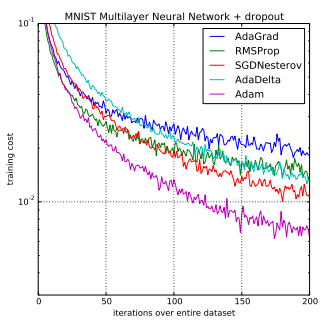
\includegraphics[width=0.70\textwidth]
            	{./Figuras/MLM/optimizers.png}
            
            \caption{Behavior of optimizers for MLP trained with \textit{Backpropagation}.}\caption*{  Source: \cite{MLM} }    \label{fig:otimizadores}}
        
            \end{figure}
            
    \subsection{Recurring Networks: The GRU model}\label{sec:GRU}

    The networks GRU, abbreviation of \textit{Gated Recurrent Unit},were first introduced in \cite{gru},being an adaptation of LSTM networks (Long Short-Term Memory).
    
    The LSTM networks were presented in \cite{lstm}, and use memory blocks called cells, which allow certain information to be kept on the network. The manipulation of information is made by \textit{gates} (by which the procedure is often called \textit{gating}). For these networks, there are three types of gates: i) forgetting gate, to remove information that is no longer useful, ii) input gate, to add useful information to the cell condition, and iii) output gate, to extract useful information from the cell condition. 
    
    LSTM networks allowed the resolution of more complex problems, but still had the problem of dissipating the gradient by which the memory could not maintain information of long sequences using the term of short-term memory.
    
    The GRU recurring networks solved this problem by changing the use of cell state to a hidden state with two new gates. These gates, called \textit{update gate} and \textit{reset gate} determine which information should be passed to the output and can be trained to maintain long sequence information without being dissipated of the values. 
    
    In \cite{DLB}, these gates are cited as the useful structures for solving prediction problems. In the Figure \ref{fig:gru-arch} are presented two network models, an LSTM and a GRU, indicating the gates in each one. 
         	
    \begin{figure}[ht]
    	\center{
    		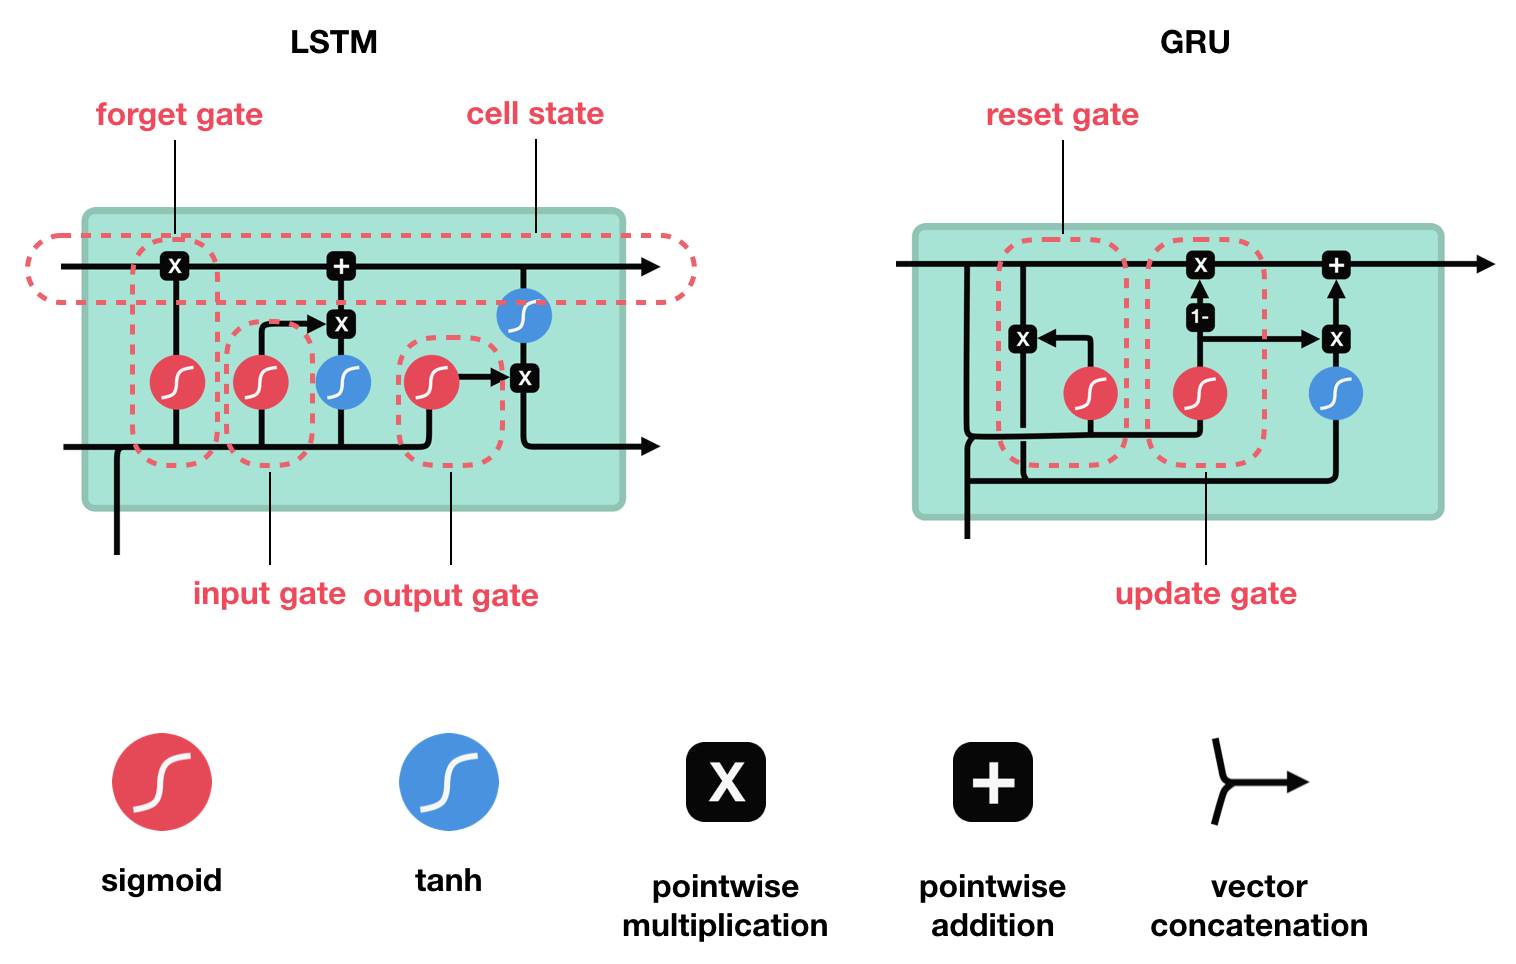
\includegraphics[width=0.80\textwidth]
    		{./Figs/10-portoes-rnns.png}
    	 	\caption{Architecture of the GRU model.}\caption*{  Source: \cite{DLB}} \label{fig:gru-arch}}
    \end{figure}
    
    The GRU networks then allowed the solution of problems with long sequences of data, solving the problem of short-term memory. So the biggest difficulty that could still arise in supervised trials was due to overfitting, by which another tool was proposed to prevent the network from memorizing beyond what was desired: the method \textit{dropout}.
    
    \subsubsection{Dropout} \label{sec:drop_fund}
    
    The \textit{Dropout} method has been introduced in \cite{dropout}, a term translated into Portuguese in the literature as abandonment, and proposes the temporary removal of some cell from the network. 
    
    In \cite{dropoutapp} has been applied \textit{dropout} was applied in the training of a neural net, in which, in each training period some cells of the entry layer are randomly disconnected and some of the hidden layers are all reconnected at the end of the training period. Thus, in each training season only a sample of the data is processed by a subset of the hidden cells.  
    
    This method seeks that the randomness of the choice of cells in each period induces a reduction in the dependence between them in the process of adjustment, making each unit generate patterns that do not depend on those learned by others. At the time of the test, all weights are multiplied by the probability that your cell has been turned off. 
    
    In \cite{dropoutapp} successful network training results are obtained with \textit{dropout} when in each season 50\% of the cells are disconnected in hidden layers and 20\% of the cells in the entrance layer.
    

    


    \chapter{Trabalhos relacionados} \label{cap:literatura}
  
Este capítulo descreve os principais trabalhos relacionados encontrados na literatura referenciada neste trabalho. A primeira seção cita a primeira referência literária encontrada na execução deste trabalho que realiza comparações de métodos de previsão de demanda. A segunda seção cita pesquisas relacionadas ao tema deste trabalho, a predição de demanda em restaurantes universitários, contendo estudos relacionados com uma parte dos métodos executados neste trabalho que são os modelos de redes neurais MLP, e o diferencial deste trabalho em relação aos outros é a inclusão de redes neurais recorrentes modernas, denominadas GRU, fundamentadas no tópico \ref{sec:GRU}. A última seção cita o maior volume de referências encontradas durantes as pesquisas de predição de demanda em geral, e que não corresponderam ao tema deste trabalho.

    \section{Trabalho de comparações de métodos de previsão de demanda.}
       \citeonline{Junior2007} Realiza um trabalho de comparação entre os métodos estocásticos (Método de suavização exponencial, modelos de Box-Jenkins) e modelos de aprendizado de máquina (Redes Neurais), ilustrados na Figuras \ref{fig: metodosPrevisaoDemanda}, os quais são usados para a previsão da demanda de produtos cosméticos distribuídos em séries temporais. Entre as Redes Neurais, encontramos redes do tipo \textit{feedforward} com o algoritmo de treino por \textit{backpropagation} que foi o principal foco no trabalho de previsão do R.U na Universidade Federal de Viçosa e na Universidade Estadual Paulista Júlio de Mesquita Filho, e que também fundamentou parte do desenvolvimento deste trabalho de predição no ICT Unifesp. Neste trabalho do autor, também são analisadas diversas medidas de performance preditivas e é feito uma análise comparativa final destas medidas entre os métodos citados.
    
    \section{Previsão de demanda em restaurantes universitários}
        No estudo estatístico feito por \citeonline{Landim2016}, foi analisada a correlação entre a temperatura e o consumo de refeições nos dias de vendas do restaurante universitário do campus ICT-Unifesp, sendo que os dados continham apenas uma pequena amostra das vendas do segundo semestre de 2016. Devido ao baixo volume de ocorrências, os dados foram submetidos à reamostragem via bootstrap. De acordo com os gráficos das amostras, identificou-se que a correlação mostrada nos gráficos da primeira metade do semestre e do período total do semestre formaram distribuições bimodais. Porém, na segunda metade do semestre formou-se uma distribuição unimodal. Portanto, concluiu-se que outras variáveis e outros modelos de análises deveriam ser utilizados para esta previsão de demanda.
        
        \citeonline{Lopes2008} faz o mesmo estudo deste cenário do ICT-Unifesp aplicado na Universidade Federal de Viçosa (UFV). Neste estudo, os dados utilizados foram somente o histórico de vendas do restaurante universitário, e nenhuma variável de ambiente foi coletada como temperatura, precipitação, número de alunos matriculados, etc. O algoritmo utilizado foi o \textit{Traincgp (Conjugate gradient backpropagation with Polak-Ribiere updates)} no software Matlab. Este algoritmo não envolve o cálculo das derivadas segundas das variáveis e converge ao mínimo da função quadrática em um número finito de iterações como cita o autor. Foram então considerados para cada nó da rede neural, o dia da semana (como segunda, terça, quarta, quinta e sexta) e cada camada dessa rede utilizando os 5 dias anteriores para cada nó (as 5 segundas anteriores, 5 terças anteriores e assim sucessivamente) e, por fim, obtido um modelo pela rede que apresentou erro máximo de 3. A rede neural aplicada neste trabalho é representada na Figura \ref{fig:mlp-lopes}.
        
        \begin{figure}[h]
        \center{
        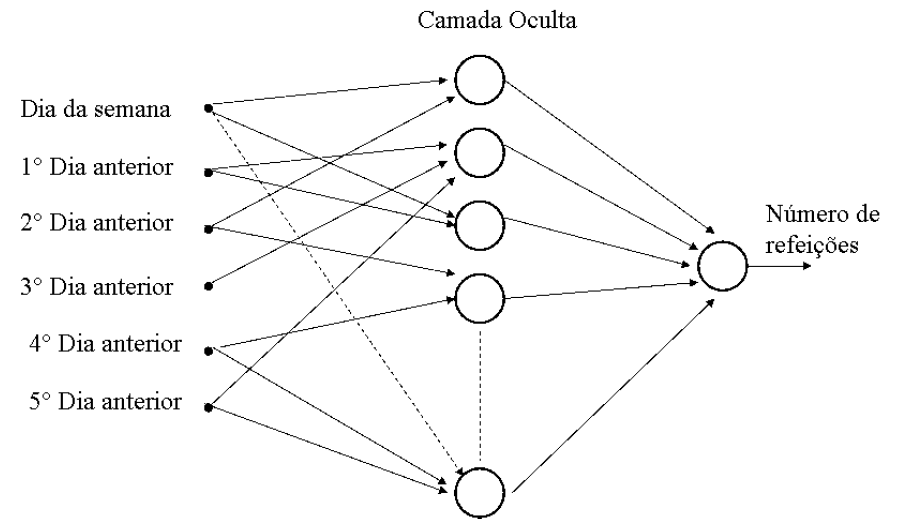
\includegraphics[width=\textwidth]
        {./Figs/15-rna-lopes.png}
        \caption{Rede Neural Perceptron de Múltiplas Camadas.}\caption*{  Fonte:\cite{Lopes2008}.}\label{fig:mlp-lopes}}
        \end{figure}
        
        \citeonline{Rocha2011} também realiza o estudo de demanda no restaurante universitário da Universidade Estadual Paulista Júlio de Mesquita Filho (UNESP), novamente com os métodos de redes neurais artificiais com backpropagation e utilizando apenas como fonte de dados (o histórico numérico das vendas realizadas), e outras variáveis intermediárias obtidas a partir deste, como médias de subconjunto de observações (médias de segundas-feiras). A única variável de ambiente coletada foi o número de feriados próximos à observação de venda. No estudo do total de dias analisados, verifica-se que em 73\% (187 dias), o método de média simples propiciou um maior erro em relação à RNA, que por sua vez ocasionou um erro maior nos 23\% (69 dias) restantes.Em se tratando de menor desperdício, observa-se que a RNA apresenta erros maiores que 50 refeições em 13 dias, enquanto o método da média simples apresenta erros maiores que 50 refeições em 58 dias, concluindo-se então que o método de RNA foi bem mais eficiente do que o cálculo de média simples utilizado pela administração do restaurante universitário. A Figura \ref{fig:rnaRocha} apresenta um esquema da rede  neural aplicada nesse trabalho. 
        \begin{figure}[h]
        \center{
        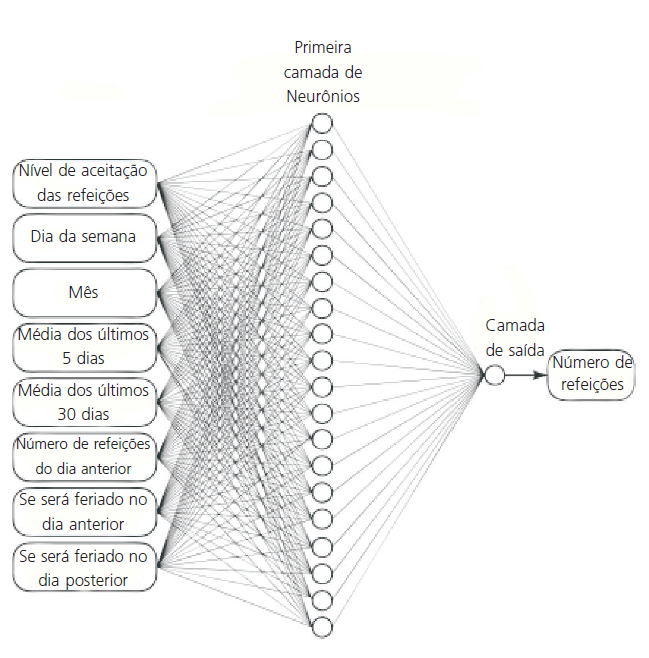
\includegraphics[width=0.8\textwidth]
        {./Figs/16-rna-rocha.png}
        \caption{Rede Neural Perceptron de Múltiplas Camadas}\caption*{ Fonte: \cite{Rocha2011}} \label{fig:rnaRocha}}
        \end{figure}
        
        Tanto o modelo apresentado em \cite{Rocha2011} quando em \cite{Lopes2008} possuem uma única camada oculta. 
      
    \section{Previsão de demanda em outros ambientes}
        \citeonline{RUAS2012} faz uma análise de previsão de demanda de energia elétrica no estado do Paraná, entre os anos de 2004 e 2006, utilizando redes neurais artificiais e máquinas de vetores de suporte. Apesar de não ser o mesmo exemplo do cenário do restaurante universitário do ICT-Unifesp, temos a distribuição dos dados de consumo coletados como uma série temporal. Nesta pesquisa de previsão de demanda de energia elétrica foi utilizada uma rede parcialmente recorrente de Elman, que permite a previsão de um passo de tempo à frente. Para que seja possível realizar a previsão para vários pontos à frente, é necessário utilizar os valores já previstos, ou seja, a saída da rede, como entradas da mesma.
        
        \citeonline{Almeida2013} analisa um cenário semelhante de demanda de energia elétrica, porém utilizando-se técnicas de previsão de demanda com Rede Neural Artificial do tipo Multilayer Perceptron combinado com lógica fuzzy que permite colocar variáveis de temperatura (entre outras) em um conjunto de regras que impactam no problema.
        
        \citeonline{Silva2010} também aplica técnicas de redes neurais para previsão de demanda de energia elétrica, com o estudo de variáveis climáticas, porém através de um modelo de MAPA SOM - (Self-Organizing Map) que é um tipo de rede neural desenvolvido para reconhecimento de padrões. Apesar de ser um modelo não supervisionado, o modelo é ideal para organizar as principais variáveis impactantes e descartáveis na previsão. O mapa som utilizado pelo autor apresenta os dados associados aos seus neurônios de forma que padrões similares encontram-se em neurônios contíguos, tendo uma organização topológica. Deste modo é possível se extrair relações abstratas entre as variáveis do vetor de dados através da sua posição nos mapas componentes, que por meio de uma escala de cores mostram a quantidade de uma variável específica em cada neurônio do mapa.
    
\chapter{Metodologia} \label{cap:metodos}


% ISSO aqui é metodologia
%Como foi evidenciado nas comunicações com a gestão do restaurante, a análise utilizada para se prever as refeições é produzir no dia da semana, como por exemplo uma segunda-feira, o consumo do mesmo dia da semana anterior (segunda-feira anterior) com acréscimo de uma margem de erro. Em geral, de acordo com o restaurante, todos os dias o mesmo trabalha com um erro e um descarte de 30\% das refeições que são trazidas e consumidas ao campus. Estima-se então que no período de 2011 - 01/08/2018 os estabelecimentos tenham tido um prejuízo de R\$1.885.938,40, e de 30\% de R\$78.386,85 no atual período de 01/08/2018 - 31/10/2018 totalizando o montante  R\$1.964.325,25. Aproximadamente 2 milhões de reais em prejuízo acumulado desde 2011.



% A obtenção dos dados do R.U do ICT Unifesp se encontra em formato de série temporal, ou seja, o consumo e vendas de refeições no R.U se distribuem em função do tempo, pelos dias letivos da universidade.
 
 
 % O cenário deste estudo analisa a sazonalidade da frequência de alunos do ICT - UNIFESP, inferida pelas grades semestrais de suas disciplinas, que consequentemente inferem na sazonalidade de consumo de refeições dentro do restaurante universitário. 
 
 
 
 
   Neste Capítulo é descrita a metodologia experimental deste trabalho, a qual consiste nos seguintes passos:
    \begin{itemize}
        \item Coleta de dados endógenos e exógenos.
        \item Transformação de cada registro de dado endógeno (os dados de consumo e vendas), em uma série temporal com intervalo de cinco dias anteriores.
        \item Análises exploratórias dos conjuntos de dados endógenos e exógenos com o conjunto de dados a serem previstos.
        \item Construção e treino dos modelos exclusivamente endógenos e dos modelos mistos, duplicados em duas fases experimentais com diferentes domínios temporais.
        \item Análises comparativas dos resultados dos modelos.
    \end{itemize}
    
    \section{Área de estudo}
       A área de estudo deste trabalho é o restaurante universitário do Instituto de Ciência e Tecnologia da Unifesp (ICT-Unifesp) em São José dos Campos. O campus do ICT foi inaugurado no ano de 2007 visando suprir as demandas científicas e tecnológicas da região do Vale do Paraíba. A Figura \ref{fig:RU_foto} apresenta um dia comum de utilização do espaço físico do restaurante unuversitário do ICT.
        
        \begin{figure}[H]
        	\center{
        	    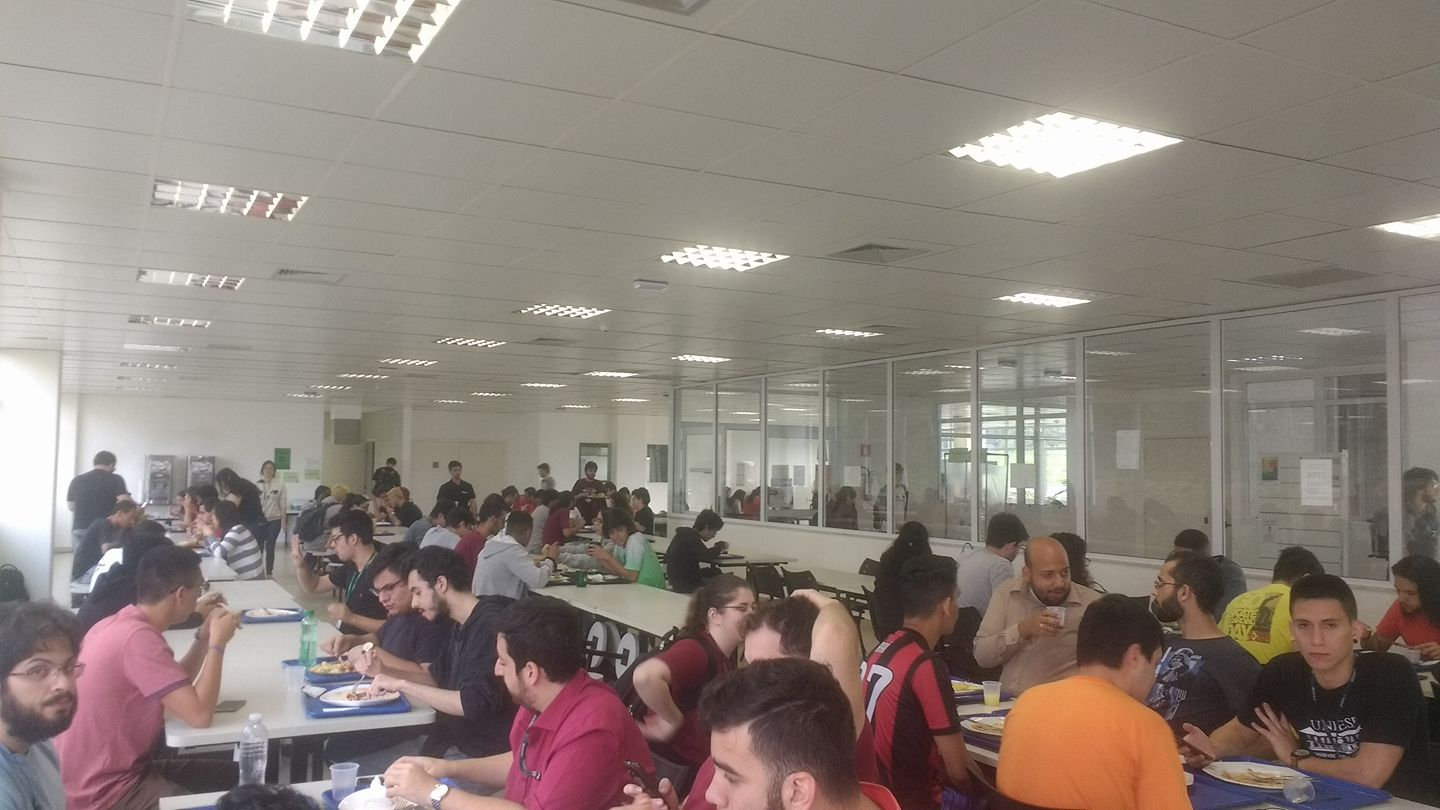
\includegraphics[width=0.7\textwidth]{./Figuras/ru_unifesp.jpg}
        	    \caption{Restaurante Universitário do ICT-Unifesp}\label{fig:RU_foto}
        	     }
        \end{figure}
    
    \section{Descrição dos dados}

    Este trabalho fará uso de dois tipos de dados, endógenos e exógenos, os quais são descritos a seguir. 
            
    Dados endógenos:  são os dados do domínio de predição neste caso. Para este problema, são as quantidades diárias de  refeições consumidas no almoço e no jantar do Restaurante Universitário (RU) do ICT-Unifesp, quantificada diariamente pela número de alunos que passam no ponto de acesso, a catraca. 
    Também são considerados dados endógenos a quantidade diária  de \textit{tickets} de refeição vendidos pelo Restaurante. Em ambos casos, as informações são tidas dos dias letivos.   Esses dados são transformados em entrada de redes neurais, em formato de série temporais.
            
    Dados exógenos: são todos os outros dados fora do domínio de predição. Para este problema, são  parâmetros derivados das datas das observações, como por exemplo o dado categórico que representa o dia da semana (segunda-feira à sexta feira), e os dados climáticos.
    
    \section{Obtenção e tratamento dos dados}
        A obtenção dos dados é realizada por meio de duas fontes distintas, sendo os dados endógenos inteiramente fornecidos através do setor de tecnologia da informação do ICT Unifesp, parte dos dados exógenos da data de registro dos dados endógenos coletados, e a parte restante dos dados exógenos, os dados climáticos, são obtidos através da uma estação meteorológica mais próxima ao ICT Unifesp, localizada na cidade de Taubaté-SP.
        
	    \subsection{Dados endógenos} \label{subsec:coleta_endogenos}
        	Os dados históricos de consumo no restaurante foram retirados do atual sistema banco de dados de refeições subsidiadas do Hospital São Paulo, que gerencia os dados dos refeitórios de todos as unidades da Unifesp. Apenas alguns funcionários autorizados têm acesso ao banco de dados da instituição, portanto para coletar tais dados o presente trabalho obteve uma autorização com a direção do campus ICT-Unifesp. Foram solicitados  os dados de consumo apenas para os discentes de graduação, visto que  o banco de dados ainda possui as informações de consumo de docentes, alunos de pós-graduação e visitantes, porém claro com menor relevância em termos quantitativo. Além disso, o padrão de consumo destes outros estratos do meio acadêmico pode influenciar  o processo de predição das demandas trazendo tendências diferentes. Na tabel \ref{table:dadosrestaurante}.
    
        	\begin{table}[!ht]
        	    \centering
        	    \caption{Formato original dos dados originais obtidos pelo restaurante universitário}
                \rowcolors{2}{gray!25}{white}
                \begin{tabular}{l|l|l}
                    \hline
                    DATA                  & (19/12/2017) & (18/12/2017) \\ \hline
                    VENDAS CAFÉ           & 0            & 0            \\
                    VENDAS ALMOÇO         & 24           & 71           \\
                    VENDAS JANTAR         & 0            & 0            \\
                    VENDAS REFEIÇÃO      & 24           & 71           \\
                    TOTAL VENDAS          & 24           & 71           \\
                    ENTR. CAFÉ            & 0            & 0            \\
                    ENTR. ALMOÇO          & 42           & 70           \\
                    ENTR. JANTAR          & 3            & 24           \\
                    TOTAL ENTR. REFEIÇÃO & 45           & 94           \\
                    TOTAL ENTRADA         & 45           & 94           \\ \hline
                \end{tabular}
               
                \label{table:dadosrestaurante}
            \end{table}
            
            Após a coleta, os dados de consumo do restaurante foram transformados em um processo de aproximação por uma série temporal, para um intervalo de cinco dias, e em cada registro de venda  acrescentados cinco novos atributos contendo os valores passados, deste mesmo atributo, em um intervalo de cinco dias anteriores. Este processo adapta o conjunto de dados para o processo de memorização das entradas, estruturando o formato compatível de leitura de dados nos modelos de redes neurais aplicados.
            
            A Tabela \ref{table:transformacaodadosrestaurante} exemplifica a nova estrutura de um registro de dado do restaurante, com um intervalo temporal de cinco dias anteriores. Nota-se que o valor de consumo da data 20/04/2017 foi removido do conjunto de dados, por se tratar o valor supervisionado a ser previsto, dado que o processo de aprendizado das redes neurais utilizam apenas dados no passado, a partir de um dia anterior.
            
            \begin{table}[!ht]
                \centering
                \rowcolors{2}{gray!25}{white}
                \begin{tabular}{l|l}
                \hline
                    DATA                  & (19/12/2017) \\ \hline
                1 DIA ANTERIOR    & 500        \\
                2 DIAS ANTERIORES & 00                            \\
                3 DIAS ANTERIORES & 300                            \\
                4 DIAS ANTERIORES & 200                            \\
                5 DIAS ANTERIORES & 100                          \\ \hline 
                \end{tabular}
                \caption{Transformação dos registros do restaurante em uma série temporal.}
                \label{table:transformacaodadosrestaurante}
            \end{table}
           
        \subsection{Dados exógenos} \label{subsec:coleta_exógenos}
            Os dados exógenos correlacionados com o consumo se dividem em dois tipos principais, dados climáticos coletados de estações meteorológicas próximas ao ICT-Unifesp, e dados derivados das datas dos registros de consumo.
    
      	 Em relação as variáveis climáticas utilizadas como dados exógenos, foram considerados parâmetros que possam afetar o consumo de refeições de forma indireta, como temperatura média ambiente, pressão atmosférica, umidade e velocidade do vento. Tais parâmetros podem ser obtidos de forma gratuita pelo BDMEP - Banco de Dados Meteorológicos para Ensino e Pesquisa, pertencente à instituição pública INMET - Instituto Nacional de Meteorologia, pertencente ao Ministério da agricultura, pecuária e abastecimento. É necessário um cadastro na plataforma do INMET \footnote{\url{http://www.inmet.gov.br/portal/index.php?r=bdmep/bdmep}} para a obtenção dos dados. A instituição contêm dados registrados de forma digital desde 1961 no país inteiro, os dados históricos referentes a períodos anteriores a 1961 ainda não estão em forma digital e, portanto, estão indisponíveis no BDMEP. Importante ressaltar que o BDMEP leva 90 dias para registrar cada nova data. 
            	
     	  Além dos dados ambientais, também foram gerados dados exógenos a partir dos dados de consumo coletados. A informação de data contida nos índices dos registros dos dados endógenos, foi derivada em diversas informações que representam o comportamento de consumo em relação à sazonalidade da frequência dos alunos influenciada pelas agendas de atividades acadêmicas.\\
            	Os seguintes parâmetros foram definidos:
            	\begin{itemize}
            	    \item Semestre 1 ou 2 em formato categórico e binário;
            	    \item Dia da semana em formato categórico e binário;
            	    \item Distancia em dias até o registro anterior e posterior;
            	    \item Avanço do semestre em escala percentual;
            	    \item Avanço do mês em escala percentual.
            	\end{itemize}
            	
            	O consumo distribuído em uma janela de cinco dias para entrada nas redes MLP seguiu padrão semelhante com os trabalho de previsão de demanda em R.U realizados por \citeonline{Lopes2008} e \citeonline{Rocha2011}, ilustrado na Figura \ref{fig:mlp-lopes}. Por fim, a Tabela \ref{table:dataset_final} representa o conjunto de dados estruturados e preparados para o processo de divisão em domínios de treino, validação e teste para o treino dos modelos.

       \begin{table}[!ht]
            \centering
            \rowcolors{2}{gray!25}{white}
            \begin{tabular}{c|c|c} \hline
                \multicolumn{3}{c}{ Estrutura final do conjunto de dados indexados por data: } \\
                \hline
                identificador &	nome da variável					&tipo de variável\\ 
                \hline
                0&	SEMESTRE\_1					&int64 \\
                1&	SEMESTRE\_2					&int64\\
                2&	SEGUNDA						&int64 \\
                3&	TERCA						&int64 \\
                4&	QUARTA						&int64 \\ 
                5&	QUINTA						&int64 \\ 
                6&	SEXTA						&int64 \\ 
                7&	DISTANCIA\_DIA\_ANTERIOR	&	int64 \\ 
                8&	DISTANCIA\_DIA\_POSTERIOR	&	int64 \\
                9&	PERC\_CONCLUSAO\_SEM		&	float64 \\
                10&	PERC\_CONCLUSAO\_MES		&	float64 \\
                11&	PRESSAO\_ATMOSFERICA		&	float64 \\
                12&	TEMPERATURA					&float64 \\ 
                13&	UMIDADE						&int64 \\
                14&	VENTO						&float64\\ 
                15&	VENDAS\_ALMOCO				&int64 \\
                16&	VENDAS\_ALMOCO\_1			&	int64 \\ 
                17&	VENDAS\_ALMOCO\_2			&	int64 \\
                18&	VENDAS\_ALMOCO\_3			&	int64\\ 
                19&	VENDAS\_ALMOCO\_4			&	int64 \\
                20&	VENDAS\_ALMOCO\_5			&	int64 \\ 
                21&	ENTR\_ALMOCO				&	int64\\
                22&	ENTR\_ALMOCO\_1				&int64 \\
                23&	ENTR\_ALMOCO\_2				&int64 \\
                24&	ENTR\_ALMOCO\_3				&int64 \\ 
                25&	ENTR\_ALMOCO\_4				&int64 \\
                26&	ENTR\_ALMOCO\_5				&int64 \\
                27&	ENTR\_JANTAR				&	int64 \\ 
                28&	ENTR\_JANTAR\_1				&int64\\
                29&	ENTR\_JANTAR\_2				&int64 \\ 
                30&	ENTR\_JANTAR\_3				&int64 \\ 
                31&	ENTR\_JANTAR\_4				&int64 \\
                32&	ENTR\_JANTAR\_5				&int64\\
              \hline
            \end{tabular}
            \caption{Estrutura final do conjunto de dados indexados por data}
            \label{table:dataset_final}
        \end{table}
        Por fim, a Tabela \ref{table:dataset_final} representa o conjunto de dados estruturados e preparados para o processo de divisão em domínios de treino, validação e teste para o treino dos modelos.
        
	\subsection{Pré-processamento}
        Na etapa de pré-processamento é realizada a transformação dos dados endógenos em séries temporais, de comprimento de cinco dias, normalização com remoção de \textit{outliers}, e aplicação de escala 0 a 1, para que todos os dados correspondam à um mesmo domínio de aprendizado. Após a conclusão destas etapas, o conjunto de dados foi preparado para as fases experimentais 1 e 2, que realizaram uma divisão do conjunto final de dados em intervalos temporais distintos. Apesar da distribuição dos dados se apresentarem em datas em função do tempo se classificando em um modelo de série temporal, assume-se a hipótese que o comportamento dos mesmos também é impactado por relações causais com outros variáveis exógenas, como recesso acadêmico, feriados, eventos, precipitações intensas que causam trânsito local e impactam na logística e frequência do público, entre outras variáveis de causas menos aparentes
    
        \subsection{Tratamento dos dados para entrada nos modelos}
         	Os dados endógenos, após estruturados na tabela final do conjuntos de dados, passam pelas seguintes transformações:
         	\begin{itemize}
                \item	Calculo do desvio padrão de cada vetor de atributos, e normalização dos valores máximos para o teto de 3x o desvio padrão, e mínimo de 0; 
                \item	Transformação dos dados em escala de 0 e 1.
            \end{itemize}
            Os dados exógenos não passam pela transformação em série temporal, portanto os mesmos foram tratados de acordo com os passos:
            \begin{itemize}
                \item	Transformação dos dados em escala de 0 e 1;
                \item	Os parâmetros categóricos binários (dias da semana e semestre) já estão escalados por serem categorias binárias.
            \end{itemize}
    	\subsection{Fases Experimentais} \label{subsec:fases_experimentais}
            O processo experimental foi realizado em dois roteiros distintos de divisão do domínio temporal do conjunto de dados, e os resultados obtidos entre as duas fases foram comparados.
            
            O conjunto de dados contemplando o período de 2017 a 2019, foi dividido em conjunto de treino, validação e teste da seguinte maneira: 
            
            \paragraph{1º Fase com validação no 1º semestre de 2018 e teste no 1º semestre de 2019}
                Neste roteiro, o semestre de validação que compõe o conjunto de dados para o treino \textit{backpropagation} das redes neurais contempla o primeiro semestre de 2018 e o conjunto de teste contempla o primeiro semestre de 2019.
                Os dados de 2017 contemplando o 1º e 2º semestre, e 2018 contemplando o 2º semestre, foram usados para treino. Os resultados obtidos nesta divisão foram usados para validar a hipótese de que os modelos aprendem especificamente a sazonalidade de consumo no primeiro semestre, se saindo melhor nos testes realizados no primeiro semestre de 2019, em comparação aos outros modelos treinados com validação no ano todo de 2018.
                Portanto, o conjunto de dados da primeira fase contempla o seguinte domínio:
            \begin{itemize}
                    \item Conjunto de treino dos modelos, contemplando o primeiro e segundo semestre de 2017, e segundo semestre de 2018;
                    \item Conjunto de validação dos modelos, contemplando o primeiro semestre de 2018;
                    \item Conjunto de teste dos modelos, contemplando o primeiro semestre de 2019.             
            \end{itemize}
            
            \paragraph{2º Fase com treino em 2017, validação em 2018 e teste em 2019}
                Nesta fase, os conjuntos foram divididos conforme sua descrição e o melhor modelo encontrado passa por uma última etapa de teste no domínio da primeira fase (teste somente no primeiro semestre de 2019).
                As métricas obtidas neste teste foram comparadas com o melhor modelo da primeira fase.
    
    \section{Definição e treino dos modelos}
            %\paragraph*{Sobre a necessidade de implementar modelos mistos}
                No conjunto de dados deste trabalho, os dados obtidos se dividem em dados temporais e endógenos (tal que cada registro de consumo e venda trás a informação de seu domínio em um intervalo temporal de cinco dias anteriores) e dados discretos e exógenos, sendo variáveis categóricas de data para cada registro, e variáveis climáticas.
                
                Portanto foi necessária a implementação de modelos específicos para entradas temporais e modelos específicos para as entradas discretas.
                Para a saída final foi implementado um comitê de redes neurais endógenas e exógenas, com um neurônio perceptron na saída, recebendo os dois valores dos modelos endógenos e exógenos para a regressão das saídas das duas redes ao valor que será a predição do consumo.
         	\paragraph{Modelos endógenos}
         	\begin{itemize}
                \item	Desenvolvimento das redes perceptron de baixa profundidade para avaliar o aprendizado da rede;
                \item	Aumento da profundidade da rede e avaliar as mudanças da função de perda RMSE; 
                \item	Implementação e avaliação dos modelos com redes recorrentes GRU, conforme a Figura. \ref{fig:gru-arch} que são especialmente desenvolvidos para o aprendizado com memorização de dados, e no caso deste trabalho, podem memorizar as sazonalidades semanais de consumo (em um intervalo de cinco dias).
            \end{itemize}
            \paragraph{Modelos Mistos : Endógenos e Exógenos}
                \begin{itemize}
                    \item Para os dados temporais (consumo e venda) utilizou-se os melhores modelos endógenos dos experimentos anteriores para as entradas endógenas. 
                    \item Para os dados discretos e categóricos adaptou-se a entrada destes dados para rede perceptron
                    \item  Concatenou-se a saída das duas redes neurais em um perceptron criando um comitê de redes neurais para obter a saída final prevista.
                \end{itemize}
            
	\subsection{Hiper parâmetros : Função de ativação e otimizador}
        Conforme fundamentado no Capítulo \ref{cap:teoria} na Seção \ref{sec: perceptron}, a função de ativação dá a capacidade do perceptron, quando conectado em rede, de resolver problemas lineares e não lineares, agregando adaptação e improviso ao resolver programas que não estão contidos em seus dados de alimentação.
        Portanto para as camadas ocultados das redes neurais MLP desenvolvidas será aplicada a função ReLu e para o neurônio de saída será aplicada a função linear, e o otimizador de treino realiza a função de otimizar o tempo de convergência do reajuste dos pesos à valores ideais, sendo escolhido o otimizador ADAM com taxa de aprendizado definido em 0,001.

    \section{Teste e Métricas de avaliação}
       As principais métricas de avaliação dos modelos são a Raiz do Erro Quadrático Médio ou em inglês \textit{Root Mean Squared Error} (RMSE), O coeficiente de correlação de Pearson (R), e o coeficiente "chi-quadrado" definido como $R^2$. Estas métricas estatísticas foram utilizado nas etapas de teste para avaliar a proximidade das predições do modelo com o comportamento real de consumo. As equações \ref{eq:RMSE} e \ref{eq:Pearson} apresentam a formulação para o RMSE e o coeficiente de Pearson (R), respectivamente.
       
       \begin{equation}
           RMSE = \sqrt{\frac{1}{n}  \sum_{i=1}^n (x_i^{est} - x_i^{obs})^2}
           \label{eq:RMSE}
       \end{equation}
       
       \begin{equation}
           R = \frac{\frac{1}{n}  \sum_{i=1}^n (x_{est} - \bar{x}_{est}) * (x_{obs} - \bar{x}_{obs})}{\sigma_{est} * \sigma_{obs} }
           \label{eq:Pearson}
       \end{equation}
       
       Onde “est” são os valores estimados; “obs” são os valores reais; n é o numero de amostras ; $\sigma$ é o desvio padrão; R é a correlação linear; $\bar{x}$ é a média de x. Avaliou-se também os erros positivos e negativos entre os valores previstos e reais, para representar quantas refeições seriam descartadas e quantas estariam em falta se a produção de refeições fosse de acordo com as predições do modelo.
       
  % ----------------------------------------------------------
  % \chapter{METODOLOGIA}
  % ----------------------------------------------------------
    \chapter{Results} \label{cap:resultados}


%%Nos parâmetros de previsão de consumo no ICT Unifesp, a função ReLu ganha destaque para utilização em neurônios nas camadas ocultas da rede neural, por ser simples e eficiente para a aplicação nos experimentos, visto que na fase feed-forward tem efeito parecido com a função identidade, e na fase feed-backward durante o reajuste dos pesos pelo otimizador, conforme ilustrado na Figura \ref{fig:ReLu}, sua derivada produz efeito degrau zerando valores negativos e sendo adequada na aplicação do domínio destes parâmetros, visto que todas as variáveis endógenas e exógenas utilizadas como parâmetros de predição, como por exemplo pressão atmosférica, vendas e consumo de dias anteriores, datas, entre outros, não possuem valores negativos. Já a função linear ganha destaque para aplicação no neurônio de saída que determina o consumo previsto para uma data no futuro, pois na fase feed-backward do reajuste dos pesos pelo algoritmo de treino backpropagation, a derivada da função linear se torna zero, fazendo com que o algoritmo de treino transforme apenas os pesos sinápticos dos parâmetros de entrada os pesos sinápticos dos neurônios nas camadas ocultas da rede, sem interferir no neurônio de saída.

This chapter describes the main experimental results obtained during this research. As described in Chapter 4, the experiments were conducted in two phases. However, we have chosen to present in this chapter only the main results obtained. The other results are available in the Annexes to this document. The first sections introduce the organization of the data, a brief analysis of the variables and the experimental protocol, respectively.

\section{Organization of the data set}
%\TODO{descrever, nessa seção, como os dados foram organizados em treino, validação e teste}

    The data collection procedure was carried out according to the methodology of Section \ref{subsec:coleta_endogenos} for endogenous data, and according to the steps of Section \ref{subsec:coleta_exógenos} the exogenous data were obtained.
    Both sets of data collected were structured according to the Table \ref{table:dataset_final}, containing a time interval of records, from April 12, 2017 (2017-04-12) for the first record to December 16, 2019 (2019-12-16) for the last record, totaling 514 records of meal consumption on school days.
    
    According to the methodology defined in Section \ref{subsec:fases_experimentais}, this data set with a total of 514 records has been duplicated to 2 distinct experimental phases, each with a specific organization of the data set. The data set of the first experimental phase was organized according to the Figure \ref{fig:case1_timeline}. This phase has the validation set exclusively contemplating the first semester of 2018, indicating that the first semester of 2018 could present a consumption and sales movement similar to the first semester of 2019, being the ideal one for tests involving only the first semester of the test set.

    \begin{figure}[htb]
        	\center{        		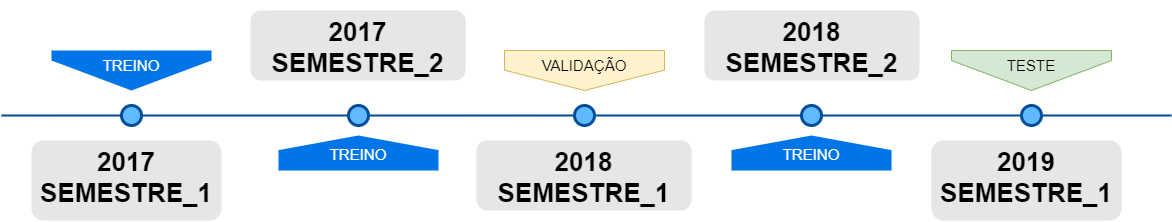
\includegraphics[width=1.0\textwidth]{./Figuras/resultados/case1_timeline.png}
        	 	\caption{Time domain of phase 1.} \label{fig:case1_timeline} }
        \end{figure}
    For the second phase the data set was organized according to the Figure \ref{fig:case2_timeline}. For this phase the selected validation set contemplated the entire school year of 2018, while for the model testing experiments the selected data contemplated the entire school year of 2019.
    
    \begin{figure}[H]
        	\center{        		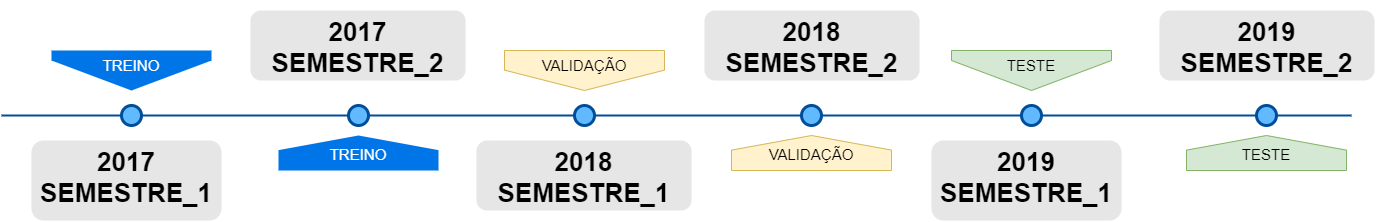
\includegraphics[width=1.0\textwidth]{./Figuras/resultados/case2/case2_dominio.png}
        	\caption{Time domain of phase 2} \label{fig:case2_timeline} }
        \end{figure}
   
    %\paragraph{Dificuldades encontradas e resolvidas}
    \subsection{Manipulation and pre-processing of the data set}
    
    Seeking to organize the raw data obtained for its subsequent application in the models, some peculiarities were found. The first difficulty found in the experiments was an anomalous behavior of the forecast results for model RNN\_ENDO\_2. The blue line in Figure \ref{fig:pandas_wrong_indexing} represents a meal forecast of model  RNN\_ENDO\_2, and the red line real consumption values of the first half of 2019. In this way, it was possible to observe that in both sets (real and predicted) this behavior was present. 
    
    \begin{figure}[!htpb]
    	\center{
    		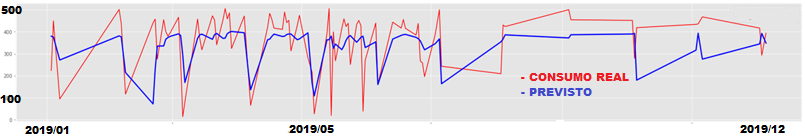
\includegraphics[width=1.0\textwidth]{./Figuras/resultados/pandas_wrong_indexing.png}
    	\caption{Result of  RNN\_ENDO\_2 model obtained on the data set randomly ordered over time.} \label{fig:pandas_wrong_indexing} }
    \end{figure}
    
    After an exploratory analysis it was discovered that the records contained an error in the indexing by date, where the date stamp was changed, that is, the days by months and vice versa. After the correction of this indexing problem the actual consumption and forecast data produced realistic results and within the expected format, as presented in Figure \ref{fig:pandas_correct_indexing},  that presents an example of prediction by model RNN\_ENDO\_2 and the real data for the lunch period.
    \begin{figure}[!htpb]
    	\center{
    		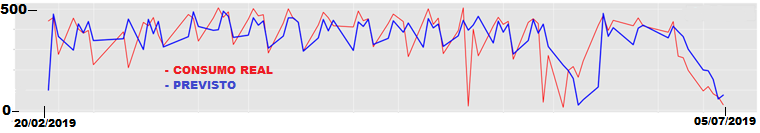
\includegraphics[width=1.0\textwidth]{./Figuras/resultados/pandas_correct_indexing.png}
    	\caption{Result of RNN\_ENDO\_2 model obtained on the data set with corrected order. } \label{fig:pandas_correct_indexing}}
    \end{figure}
              
\section{Variable Evaluation}
During this section some comments will be made about the variables characteristics that were most important to the problem, and some graphs will be presented from the statistical study done to evaluate the relationships among them. 

    \subsection{Refectory consumption estimates}
    
        The analysis of the estimation technique of consumption, performed subjectively in relation to the consumption of the previous week, uses the calculation of  30\% of production above the consumption of the fifth previous day. This estimation method is adopted to tolerate discards due to the existence of a contractual fine for lack of meals. Still, it is possible to observe that this model of  30\% more produces a linear behavior, represented by the blue line in the Figure  \ref{fig:ru_pred},  being distant from the real consumption behavior, indicated by the red line. 

        \begin{figure}[!htbp]                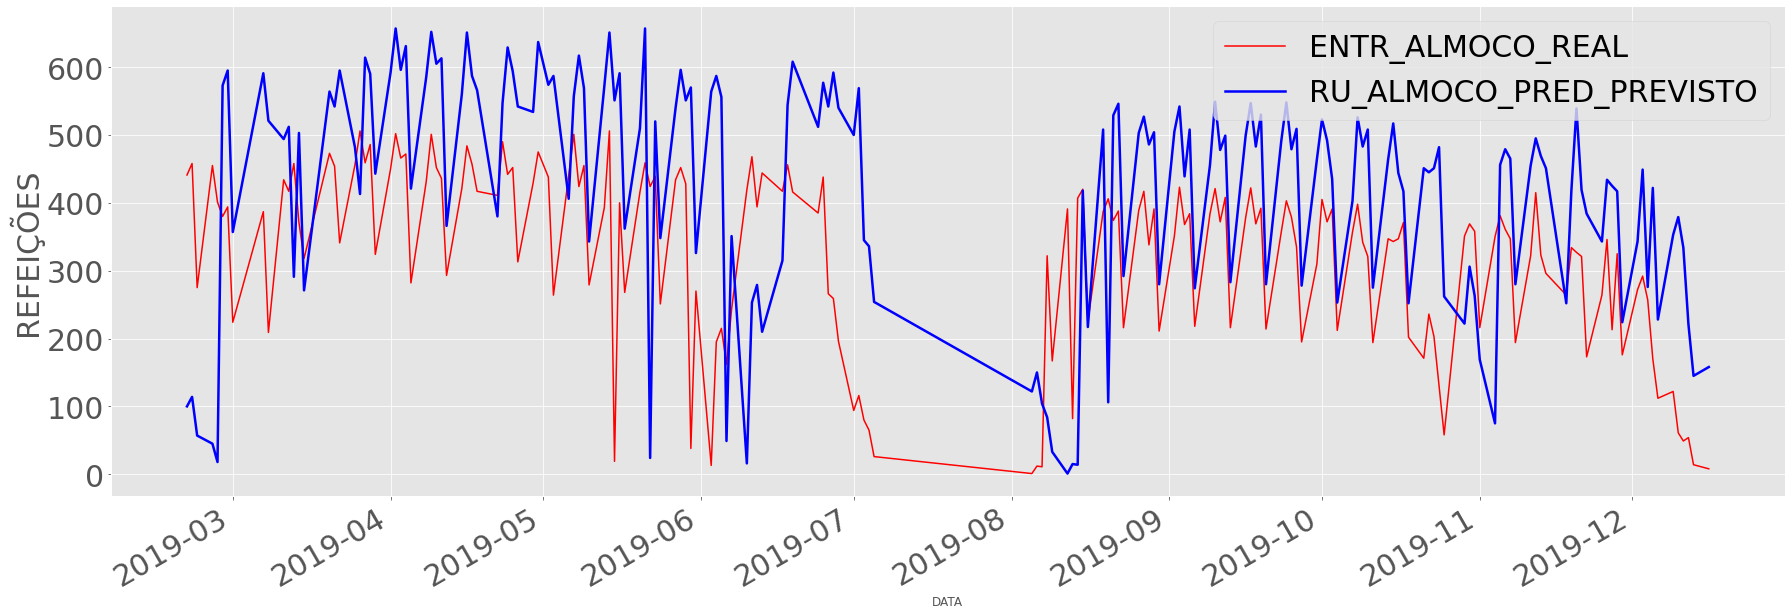
\includegraphics[width=\textwidth]{./Figuras/resultados/case1_ru_pred.png}
                \caption{Refectory estimate for 2019.} \label{fig:ru_pred} 
        \end{figure}

            
        
        Although the estimate follows the trends of falls and increases in consumption, the Figure \ref{fig:ru_pred_scatter} shows the dispersion generated between the estimate of the R.U and the actual consumption in the year 2019, showing that the linear regression (red line) has the axis totally decentralized with the function identity of the ideal estimate (represented by the imaginary diagonal formed between the origin of the graph and the top right vertex). 
        

                \begin{figure}[ht]
                    \center{                    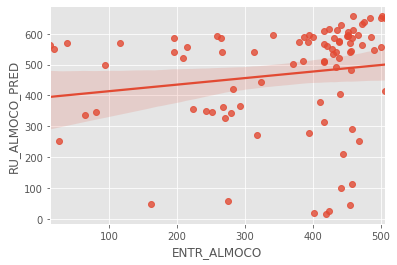
\includegraphics[width=0.6\textwidth]{./Figuras/resultados/case1_ru_pred_scatter.png}
                    \caption{Scatter plot of the refectory's estimated consumption for the year 2019.} \label{fig:ru_pred_scatter} }
                \end{figure} 

        
        
        Thus, this format of prediction also generates an error higher than 30\% in the total amount of meals discarded during the semester, caused by the oscillatory behavior of consumption, according to the table \ref{table:case2_rupred}.

            \begin{table}[!ht]
            \centering
            \rowcolors{2}{gray!25}{white}
                \begin{tabular}{c|c}
                \rowcolor{gray!50}
                \hline
                \multicolumn{2}{c}{Consumption with margin 30\% above the previous day 5}\\ \hline     
                TOTAL MEALS CONSUMED & 58653  \\
                TOTAL ESTIMATED MEALS & 76262 \\ 
                CORRELATION (r)&  0.4006 \\
                P-value & 2.0845e-08\\
                RMSE & 191.7620 \\
                SUM OF POSITIVE ERRORS & 23412 \\
               SUM OF NEGATIVE ERRORS  & -5803 \\
                AVERAGE ABSOLUTE ERROR & 133.0 \\
                ABSOLUTE ERROR AVERAGE PERCENTAGE & 205.6113\% \\  \hline 
                \end{tabular} \caption{Metrics of the refectory's estimated consumption for the year 2019}
            \label{table:case2_rupred}
            \end{table}

    \subsection{Analysis of endogenous variables}
    
        The endogenous variables are the input time parameters in the MLP and GRU models, corresponding to the consumption domain in the restaurant.
         % \newpage
        \subsubsection{Consumption of the current day in relation to the previous day's ticket sales}
        
        It is possible to notice in the Figure \ref{fig: case1_consumo_vendas_almoco} that ticket sales in the lunch period showed a different behavior in 2017 compared to the following years due to a limitation imposed by the refectory, from 2018 onwards students could purchase only 2 tickets per day. Possibly, this limitation was given to approximate the consumption behavior of 1 or 2 days after the ticket sale. This limitation can be interpreted as a management aid method for meal production and waste treatment.
        
        \begin{figure}[h]
                    	\center{                    		        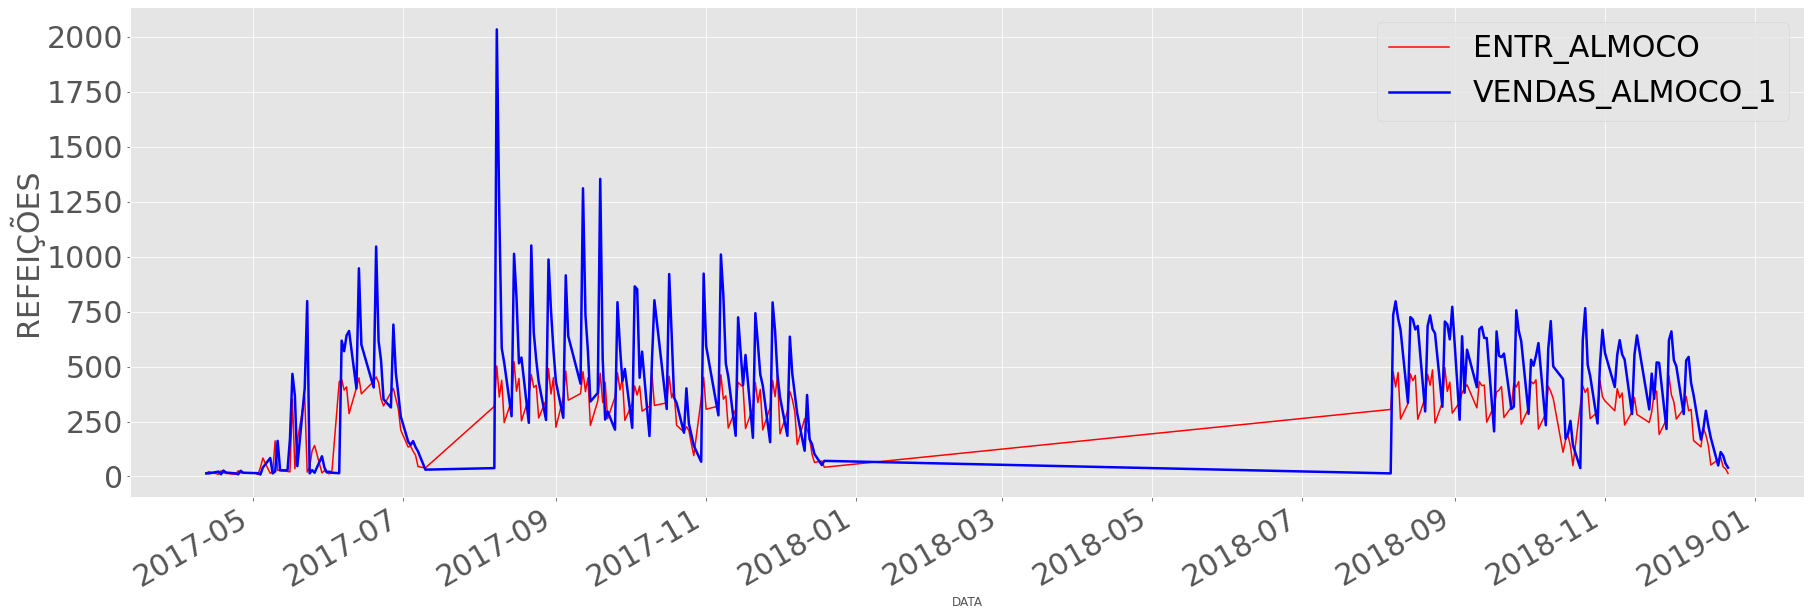
\includegraphics[width=0.8\textwidth]{./Figuras/resultados/case1_consumo_vendas_almoco.png}
                    	\caption{Correlation between consumption and lunch sales.} \label{fig: case1_consumo_vendas_almoco} 
                    	}
                    \end{figure}
	        
       Even with the \textit{outlier} value of 2000 sales in a single day, and with the new limitation on ticket purchases from 2018 onwards, consumption at lunchtime is strongly related to ticket sales in the previous day's lunch period. It is also noted that students have adapted to the limitation imposed for the use of tickets with a validity period of only two days, as the value of the correlation coefficient is approximately 72\%, as shown in the table \ref{table:case1_vendas1}.
        
 \begin{table}[!htpb]
           \centering
           \caption{Comparison of consumption with a previous day}
             \rowcolors{2}{gray!25}{white}
             \begin{tabular}{c|c}\hline
                \multicolumn{2}{c}{CONSUMPTION IN RELATION TO SALES OF 1 DAY BEFORE}\\ \hline
                CORRELATION (r) &  0.7255528038157009\\
                P-value &5.399561176138223e-41\\
                RMSE & 260.5399426736619\\
                AVERAGE ABSOLUTE ERROR & 139.0\\
                ABSOLUTE ERROR AVERAGE PERCENTAGE & 90.18\\\hline
            \end{tabular} \label{table:case1_vendas1} \end{table}
    	            

        
        There are other unscheduled factors involved, such as possible failure of sales records in the system, as well as the \textit{outlier} value of 2000 sales can be interpreted with the system and meal database migration that occurred in 2017 from the Talim unit of ICT-Unifesp to the Hospital São Paulo database. Possibly also sales were imported from the old system without the differentiation of dates.
        
        The total of meal sales at lunchtime was 242282 for all 514 entries in the data set. In this same period the actual consumption value, meaning students who effectively entered the refectory (passed through the turnstile) totaled 163752 meals. Although notorious, the difference of 78,530 meals sold above the actual consumption was not able to be investigated in this work. It should be noted that these figures were obtained from the original set of data provided by the ICT-Unifesp R.U contract inspector through an e-mail request to this inspector.


                    \begin{figure}[!htpb]
                    	\center{                    		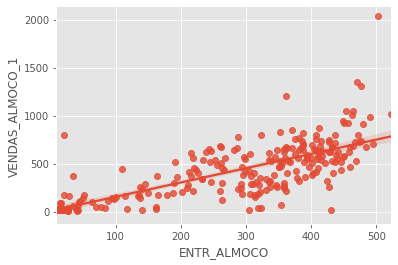
\includegraphics[width=0.7\textwidth]{./Figuras/resultados/case1_scatter_consumo_vendas_almoco.png}
                    	\caption{Dispersion graph between consumption and lunch sales.} \label{fig:case1_scatter_consumo_vendas_almoco} }
                    \end{figure}
                
                
          

            \subsubsection{Normalization and scale of \textit{features}}
            
                The process of normalization and scale is demonstrated in this Section with a \textit{feature} of sales of  \textit{tickets} from 1 previous day, because among all this is the one that has produced \textit{outliers} of greater prominence.
                The data normalization is done with the ceiling of 3x the average standard deviation, so the peak of 2000 sales was normalized to the rounded value of 1356 meals. Even with the normalization, the linear behavior of this \textit{feature} was maintained, as presented in the Figure \ref{fig:feature_sem_outliers}. 

                
                        \begin{figure}[H]
                        	\center{
                            	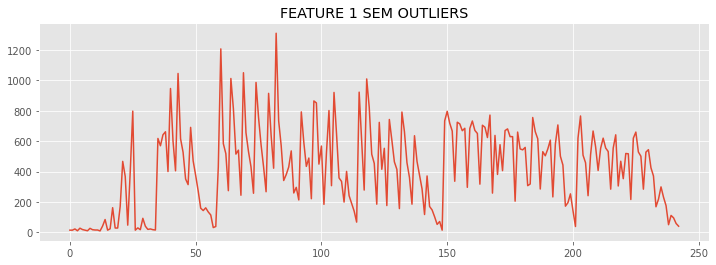
\includegraphics[width=0.9\textwidth]{./Figuras/resultados/feature_sem_outliers.png}
                            	\caption{Sales of normalized \textit{tickets} with 3x the standard deviation ceiling.}
                            	\label{fig:feature_sem_outliers}
                        	}
                        \end{figure}
                        
                        
                        After normalization, the scale was standardized from 0 to 1 in this one and as it is observed in Figure  \ref{fig:feature_sem_outliers_escalada}, the linear behavior was maintained again.
                        
                        \begin{figure}[H]
                        	\center
                        	{                    		
                            	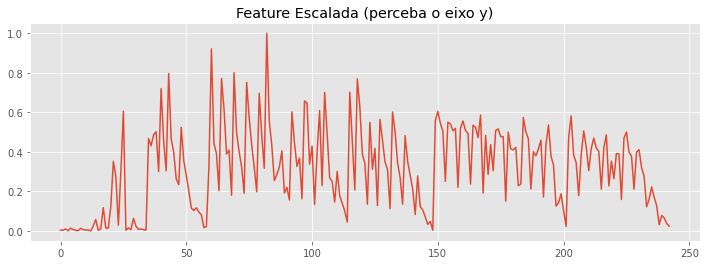
\includegraphics[width=0.9\textwidth]{./Figuras/resultados/feature_sem_outliers_escalada.png}
                            	\caption{Sales of \textit{tickets} climbing from 0 to 1.} \label{fig:feature_sem_outliers_escalada} 
                        	}
                        \end{figure}
                       
                This process of normalization and scale has been carried out for all endogenous metrics and also for climate metrics.
        	   % \newpage
        	   
                \subsubsection{The current consumption in relation to the previous day's dinner.}
                %\TODO{QUILES - esse foi um dos fenômenos mais curiosos que encontrei e que não tenho explicação pra ele, o consumo da turma da noite é muito parecido com o consumo da turma do almoço do dia seguinte}
                
                %\TODOR{Isso não foi erro de carregamento dos dados? caso esteja tudo certo, pode deixar assim. De qualquer forma, mencione isso no texto como um achado.}
                Looking to find and evaluate the possible relationship between the various metrics used, this analysis gained relevance as an anomalous and probably casual effect found among the data.
                Although the curricular schedules of students consuming meals at lunch are usually fired at students consuming dinner the night before, a clear relationship between these 2 variables can be detected.
                 This behavior can be evidenced by the congruence between the parameters, as shown in figure \ref{fig:case1_consumo_jantar} and by the high correlation obtained in the linear regression (R = 0,7655) between these 2 consumptions, presented in figure  \ref{fig:case1_consumo_jantar_scatter}. Even though it presents a relevant correlation, it was not possible to determine an evident cause for this anomalous effect found.

                
  
                \begin{figure}[H]
                	\center{
                	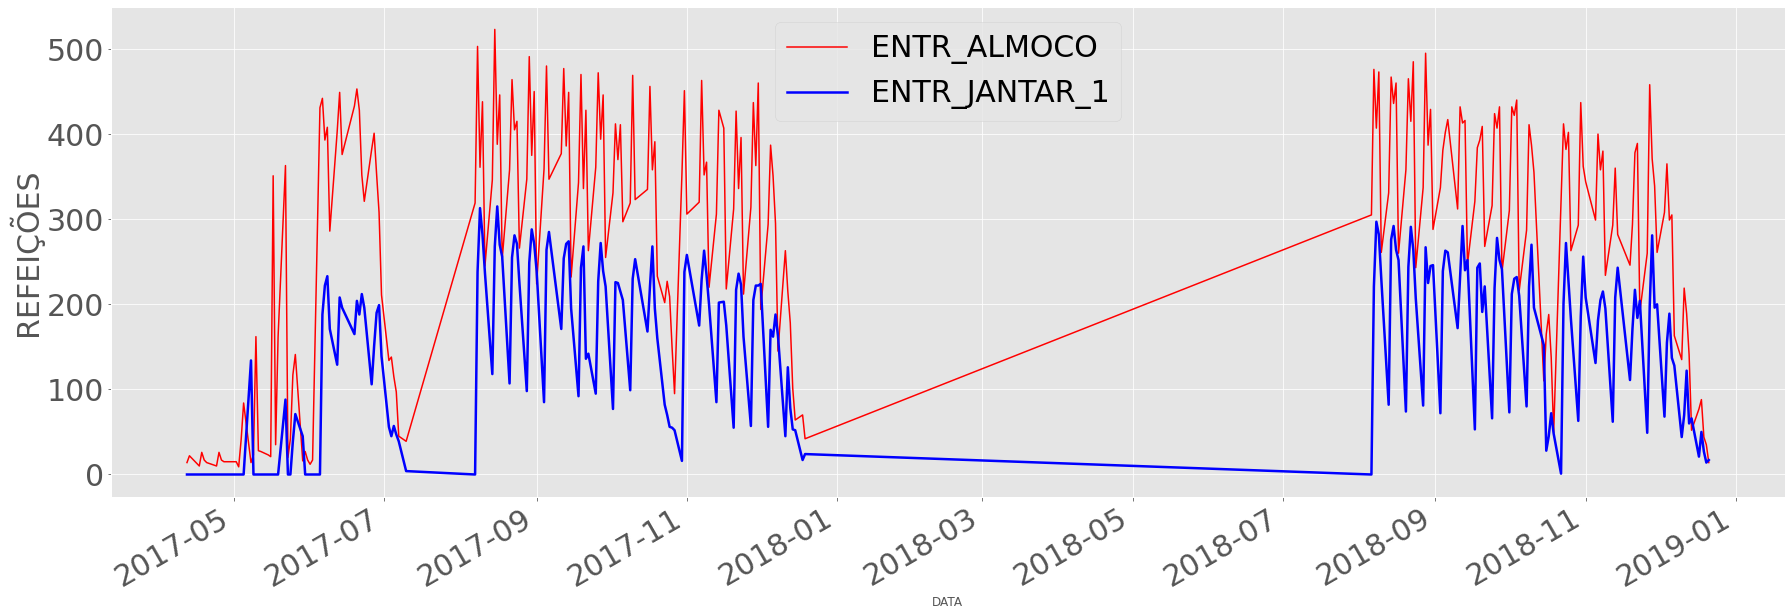
\includegraphics[width=0.8\textwidth]{./Figuras/resultados/case1_consumo_jantar.png}
                	\caption{Correlation of lunch and dinner consumption from 1 previous day.} 
                	\label{fig:case1_consumo_jantar} }
                \end{figure} 
               
                \begin{figure}[H]
                	\center{                    		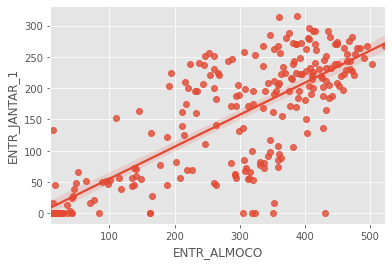
\includegraphics[width=0.8\textwidth]{./Figuras/resultados/case1_consumo_jantar_scatter.png}
                	\caption{Graph of dispersion between consumption and dinner of 1 previous day.} 
                	\label{fig:case1_consumo_jantar_scatter} }
                \end{figure}
             
            
    	    \subsection{Weekly Seasonality Analysis}
    	        The following consumption graphs from Figure 5 \ref{fig:case1_violinplot_segunda}, representing the Monday, up to figure \ref{fig:case1_violinplot_sexta}, representing Friday, are generated for the binary categorical \textit{features}, with the \textit{violin-plot} functionality in the library \textit{seaborn}, appropriate for distribution of binary categorical variables in a data set.
    	        
    	        The blue violin with the value 1 represents the distribution of consumption across the total data set.
    	        The violin with value zero can be ignored and is a standard return on the tool graph, representing the consumption complement for the day of the week considered.
    	        On Fridays, the consumption had a smaller distribution scale for the whole set 2019. It was noticeable that despite the alternation of time slots during the exchange of semesters in the year 2019, the days of Tuesday and Thursday concentrated the largest movement of consumption.
    	       %\newpage
    	      { \begin{center}    
    	        \begin{minipage}[c]{0.45\textwidth}
    	         \begin{figure}[H]
                	\center{                		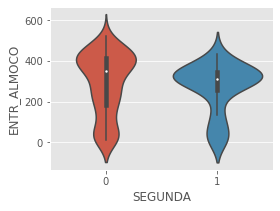
\includegraphics[width=\textwidth]{./Figuras/resultados/case1_segunda.png}
                	\caption{Gráfico de violino da distribuição do consumo na segunda feira.} \label{fig:case1_violinplot_segunda} }
                \end{figure}\end{minipage} \hfill %
                \begin{minipage}[c]{0.45\textwidth}
                \begin{figure}[H]
                	\center{                		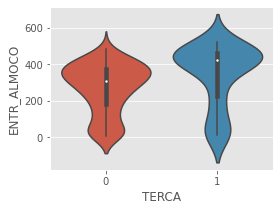
\includegraphics[width=\textwidth]{./Figuras/resultados/case1_terca.png}
                	\caption{Violin graph of Tuesday's consumption distribution.} \label{fig:case1_violinplot_terca} }
                \end{figure} \end{minipage}
                
            \begin{minipage}[c]{0.45\textwidth}
                \begin{figure}[H]
                	\center{                		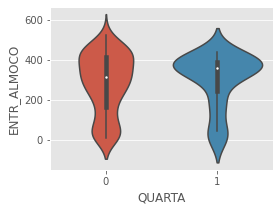
\includegraphics[width=\textwidth]{./Figuras/resultados/case1_quarta.png}
                	\caption{Violin graph of Wednesday's consumption distribution.} \label{fig:case1_violinplot_quarta} }
                \end{figure}\end{minipage} \hfill %
                \begin{minipage}[c]{0.45\textwidth}
                \begin{figure}[H]
                	\center{                		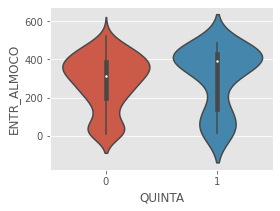
\includegraphics[width=\textwidth]{./Figuras/resultados/case1_quinta.png}
                	\caption{Violin graph of Thursday's  consumption distribution.} \label{fig:case1_violinplot_quinta} }
                \end{figure}\end{minipage} %
                        \begin{minipage}[c]{0.45\textwidth}
                \begin{figure}[H]
                	\center{                		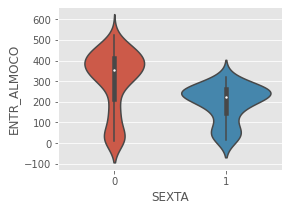
\includegraphics[width=\textwidth]{./Figuras/resultados/case1_sexta.png}
                	\caption{Violin graph of Friday's consumption distribution.} \label{fig:case1_violinplot_sexta} }
                \end{figure}
                \end{minipage} \end{center} }
    \subsection{Exogenous variables analysis}
        The exogenous variables correspond to the discrete domain parameters, which are used exclusively in mixed neural network models and are read by the MLP layers of these models.
        
        \subsubsection{The current consumption in relation to the advance of the semester.}
        
        For this analysis it was necessary to restrict the domain of analysis to 1 semester, the consumption in relation to the advance of the semester had an abrupt fall in the last days of the semester, and thus the correlation of the data sets of figures \ref{fig:case1_perc_sem} and \ref{fig:case1_perc_sem_scatter} obtained negative value.
        
                \begin{figure}[H]
                	\center{                    		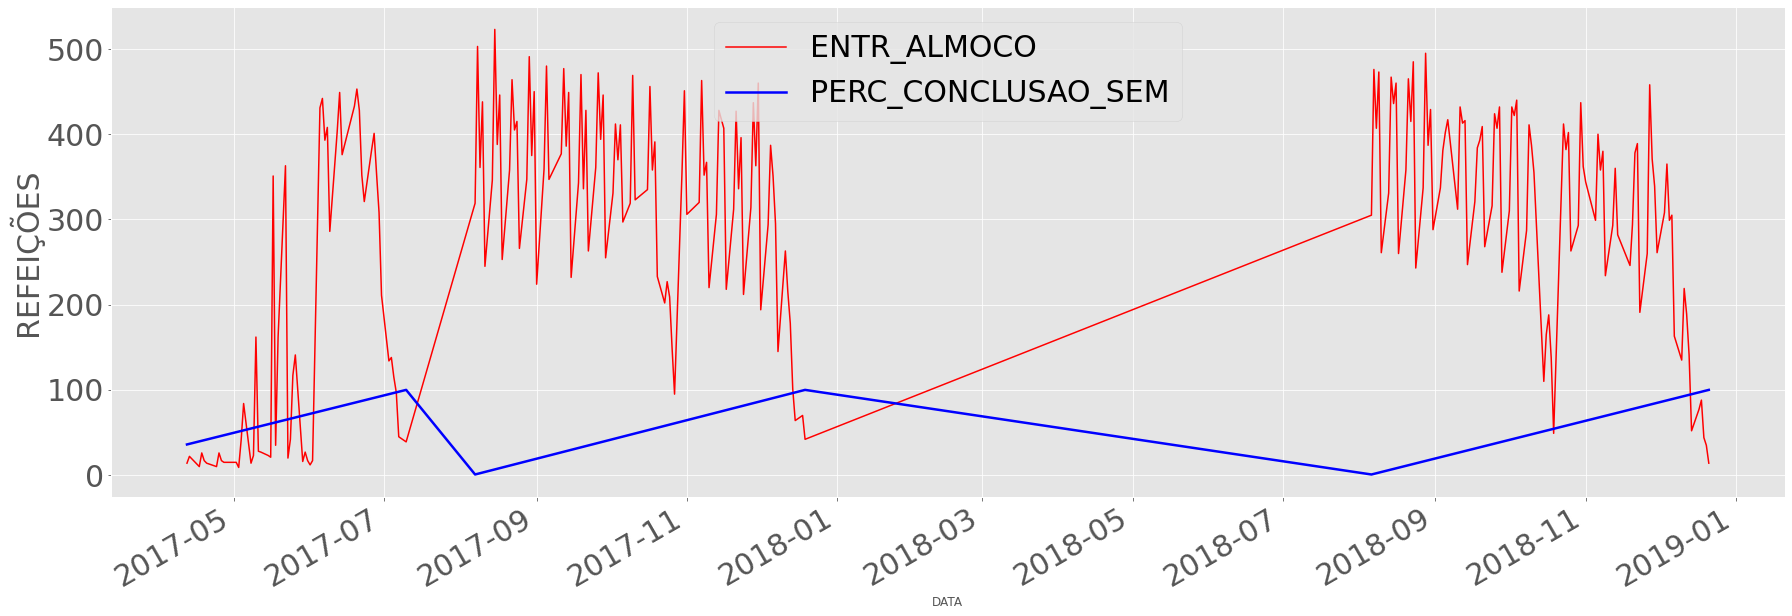
\includegraphics[width=\textwidth]{./Figuras/resultados/case1_perc_sem.png}
                	\caption{1st Phase : Relation between consumption distribution and semester's advance, Correlation (r) = -0.35.}
                	\label{fig:case1_perc_sem}
                	}
                \end{figure}  

        
                       \begin{figure}[H]
                	\center{                		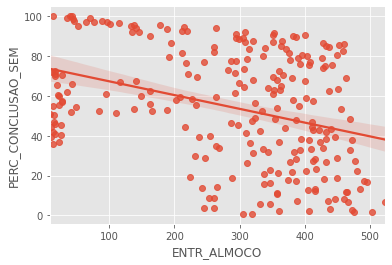
\includegraphics[width=\textwidth]{./Figuras/resultados/case1_perc_sem_scatter.png}
                	\caption{Graph of dispersion of consumption distribution as the semester progresses.} \label{fig:case1_perc_sem_scatter}
                	}
                \end{figure}
           

\section{Experimental Protocol}
%\TODO{faça um resumo sobre as duas fases e as principais diferenças entre elas. Na sequência, detalhe os detalhes do principal modelo obtido (o com melhor resultado de predição)}
    In this section will be started the experiments with the Neural Network models.
    The first experiment evaluates the learning potential of the models in predicting R.iU consumption, through a basic neural network model, by concluding that the most basic neural network topologies have learning potential about the problem.
    Then, the topology was selected and the experimental phase that brought the best results and finally it is analyzed and indicated as the final solution of the project.
    
    \subsection{Evaluation of the learning problem of meal prediction through MLP Neural Networks}
        \subsubsection{Empirical topology adjustment of the first perceptron model}
        
        The first neural net experiment performed in the first experimental phase evaluated the learning capacity of the perceptron model on the seasonality of endogenous data, referring to the domain of meal consumption in the R.U., verifying if the consumption behavior in the refectory could be learned by this type of neural net, therefore 1 initial perceptron net was defined with only 1 hidden layer containing 1 neuron for 15 input parameters (same number of endogenous parameters) and with 1 output neuron, called MLP1.
        
        The parameters endogenous correspond to an interval of 5 days prior to the consumption of meals in the lunch period, dinner and ticket sales in the lunch period.
        The model was named MLP1, its illustration can be seen in figure \ref{fig:case1_mlp1} obtained by using the NETRON tool.  
        
        \begin{figure}[H]
        \center{
        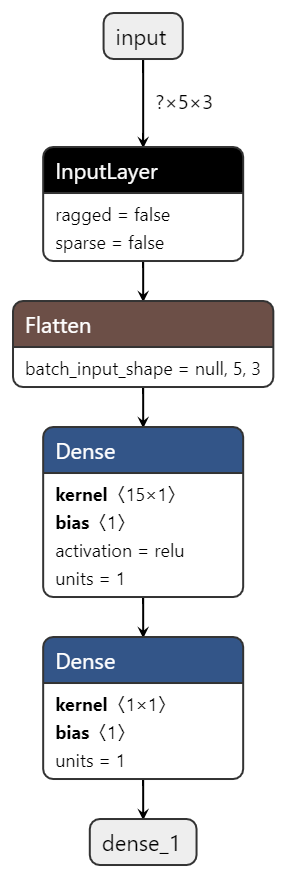
\includegraphics[width=0.3\textwidth]{./Figuras/resultados/case1_MLP1_validated.png}
        	\caption{Topology of MLP1 model, NETRON tool.} 
        	\label{fig:case1_mlp1}
        }
        \end{figure}
        
        
        Each layer of the MLP1 model corresponds to a block with title  \textbf{Dense}  in this Figure, the first edge of the figure between the \textit{input} and InputLayer shows the 3 time series of the input parameters, with an interval of 5 days each. \textbf{ENTR\_LUNCH, ENTR\_DINNER e SALES\_LUNCH}. The Flatten block converts each day of time series input into an MLP neural network input parameter, according to the conceptual model of the \citeonline{Lopes2008}work illustrated in figure  \ref{fig:mlp-lopes} which uses only 1 endogenous parameter with an interval of 5 days also. The first hidden layer of this network can be visualized in the first dense block of the figure that demonstrates the ReLu activation function of this neuron, and the number of units of this layer being 1.
        The output layer is the last block of the figure, also with 1 unit and since the activation function is linear, it is not displayed in the block description.

        
        The training of this model was executed obtaining RMSE with the value 130.62 over the validation set, in this case the first phase being the data of the first semester of 2018, and it is possible to notice in figure \ref{fig:case1_mlp1_train} that the lines of the loss and training function demonstrated an adequate training until the last training season, and as there was no application of simultaneous Validation Loss with Train Loss, the training did not produce an overfitting.
        \begin{figure}[H]
        	\center{
        	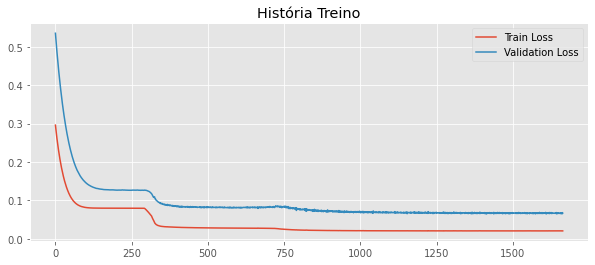
\includegraphics[width=0.8\textwidth]{./Figuras/resultados/case1_mlp1_train.png}
        	\caption{Model training graph MLP1, RMSE = 130,62}
        	\label{fig:case1_mlp1_train}
        	}
        \end{figure}
        
        Therefore, the depth of the MLP1 model was increased by obtaining the MLP2 model with topology illustrated in figure \ref{fig:case1_mlp2} and after training this model it was possible to notice the decrease of the RMSE to the value of 107.97, as observed in figure \ref{fig:case1_mlp2_train}. It is possible to realize that from the 300 training season on, the Train Loss line began to suffer a decrease in error as the Validation Loss began to gain error from the 400 season on. As the reconfiguration of the network topology produced improved results until an overfitting saturated this improvement for this topology, it was validated the hypothesis that the prediction of consumption in the refectory can be learned by simple models of Neural Networks, and therefore the research followed with the definition of new models demonstrated in the next section.
        \begin{figure}[H]
        	\center{
        		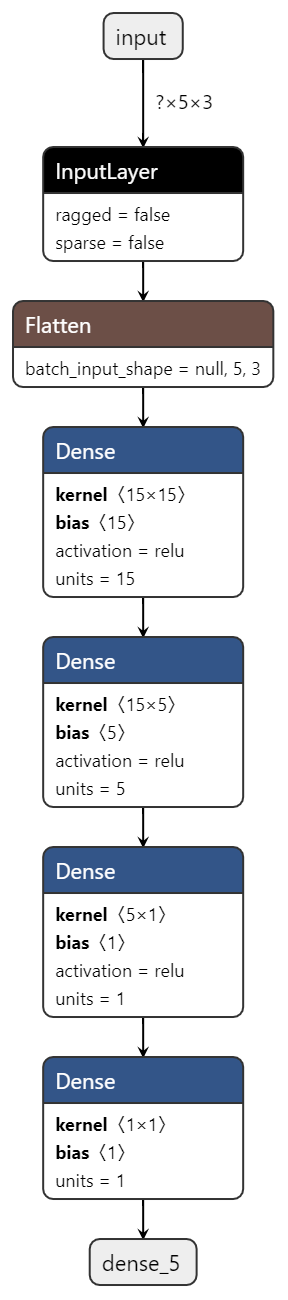
\includegraphics[width=0.3\textwidth]{./Figuras/resultados/case1_mlp2.png}
        	\caption{Model Topology MLP2.} \label{fig:case1_mlp2} }
        \end{figure}
        \begin{figure}[H]
        	\center{
        		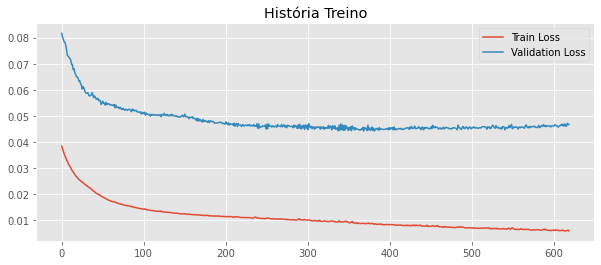
\includegraphics[width=1.0\textwidth]{./Figuras/resultados/case1_mlp2_train.png}
        	\caption{Model training graph MLP2. RMSE = 107,97.}
        	\label{fig:case1_mlp2_train} }
        \end{figure}
        
    \subsection{Topologies of best models}
    
    In this section some comments are made about the topologies of the models that obtained results presented with schematic figures of the network. For the rest of the trained models, the same procedure is done in annex \ref{cap:anexo1}.
         
        \subsubsection{Mixed Model RNN\_EXO\_1, best result in the second phase and in all the whole work}
            Interpreting the digram of the first mixed model, RNN\_EXO\_1, in figure \ref{fig:case1_rnn_exo_1} the block with the GRU title on the left in the topology figure of the model deals with endogenous (temporal) inputs, as exemplified in endogenous GRU models. The block with title \textbf{Dense} is an MLP network that receives a input with 10 parameters of 1 dimension, consequently all discrete, corresponding to the 4 climatic parameters (temperature, humidity, pressure and wind), 1 parameter for the current day of the week, 1 for the current semester and 4 calendar control parameters (distance from the previous date, later, semester advance, month advance). The output of the GRU and MLP blocks are concatenated and treated by the output MLP block.
            \begin{figure}[H]
              \center{
                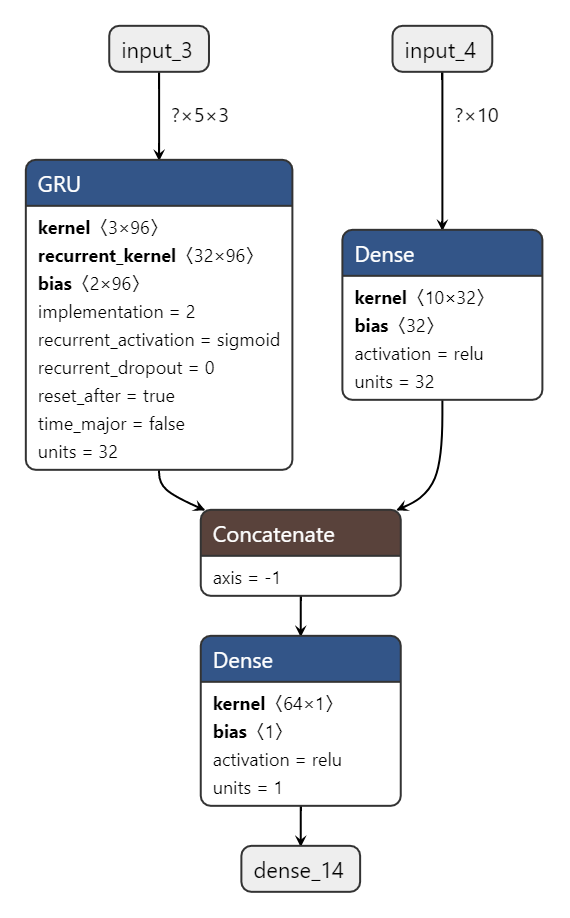
\includegraphics[width=0.7\textwidth]{./Figuras/resultados/case1_rnn_exo_1.png}
                \caption{Model Topology RNN\_EXO\_1.} \label{fig:case1_rnn_exo_1} }
            \end{figure}
        %dropout
        \subsubsection{Endogenous model GRU RNN\_ENDO\_2, best result in the first phase}
           This model was obtained through a second reconfiguration of the first GRU model, RNN\_ENDO\_1 detailed in the figure \ref{fig:case1_rnn_endo1} with the increase in unit depth of this previous model, in regressive format of 16 units in the first layer, 8 units in the second and 4 units in the third, and with the inclusion of the dropout resource based on the topic  \ref{sec:drop_fund}, the final topology is observed in figure \ref{fig:case1_rnn_endo2}. This model produced the best results in the first experimental phase, detailed in figure \ref{fig:case1_rnn_endo2_test_dates} in the next section.
            \begin{figure}[H]
              \center{
                  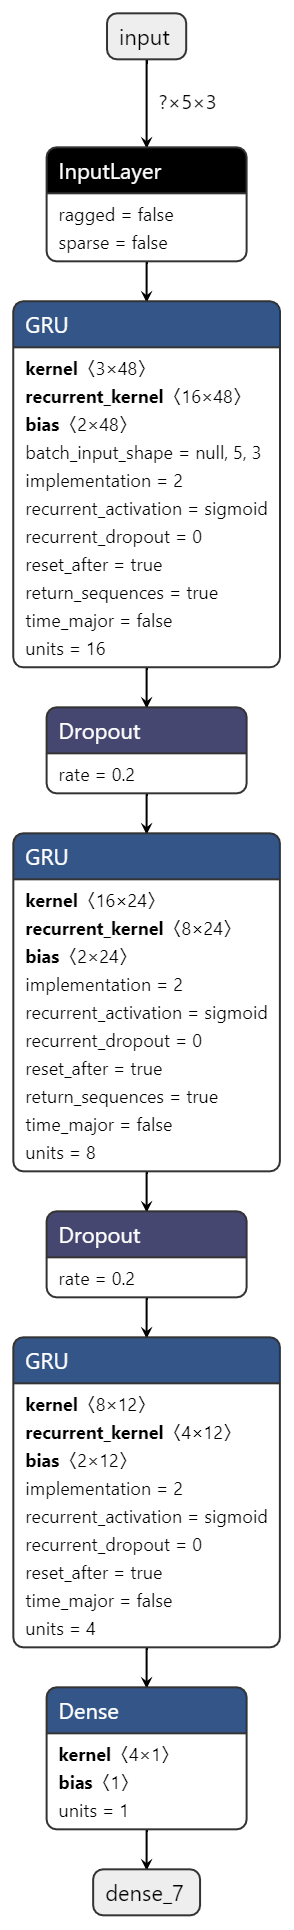
\includegraphics[width=0.24\textwidth]{./Figuras/resultados/case1_rnn_endo2.png}
                  \caption{Model Topology RNN\_ENDO\_2.} 
                  \label{fig:case1_rnn_endo2} 
              }
            \end{figure}
        
    \subsection{Main differences of results between the experimental phases}
        \paragraph{Differences between the best models}
        For the experiments of the 1st phase, the model that produced the smallest RMSE in the set of tests with advantage in all the other metrics was the endogenous model RNN\_ENDO\_2, with some prediction anomalies, as observed in figure \ref{fig:case1_rnn_endo2_test_dates}.
        \begin{figure}[H]
          \center{
            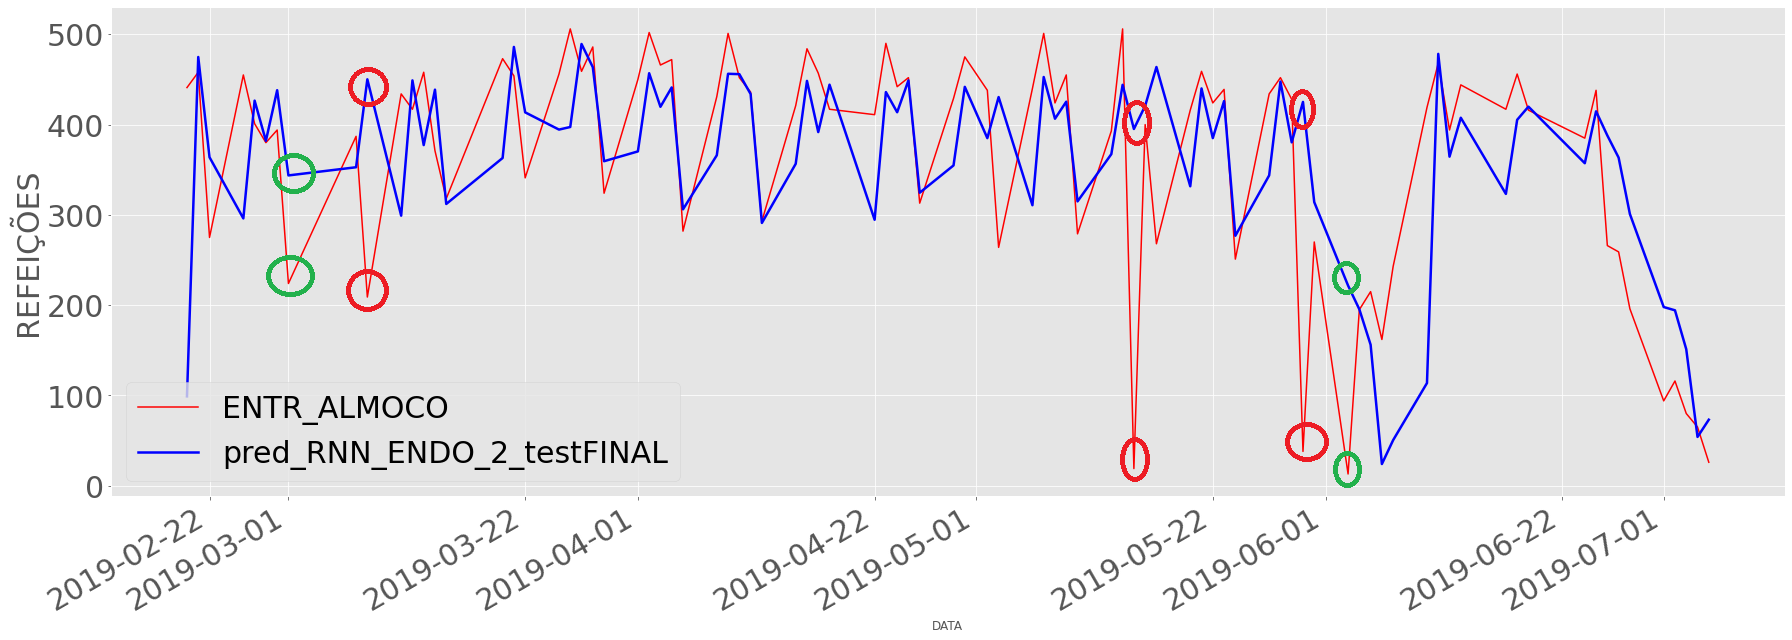
\includegraphics[width=1.0\textwidth]{./Figuras/resultados/case1_rnn_endo2_test_dates.png}
          \caption{Analysis of predictive anomalies of RNN\_ENDO\_2} \label{fig:case1_rnn_endo2_test_dates} }
        \end{figure}
        %dropout
        The green outliers represent predictions that corresponded to an upward or downward trend in consumption but with discrepant errors, and the red outliers represent predictions with an inverse trend in consumption.
        The justifications for the prediction within the trend, are found in the table \ref{table:rnn_endo_2_green}, denoting special dates that could not match the learning process of the model.
            \begin{table}[!ht]
                \centering
                \caption{Model prediction errors RNN\_ENDO\_2 in the 1st phase}
                \label{table:rnn_endo_2_green}
                \rowcolors{2}{gray!25}{white}
                 \begin{tabular}{|c|c|c|}
                 \rowcolor{gray!50}
                 \hline 
                Date & Consumption & Justification\\ \hline    
                03/01/2019 (Friday)    & 224 & Friday pre-carnival\\
                06/03/2019 (Monday)  &  13 & Monday after the student paralyzation\\ \hline 
                \end{tabular} 
            \end{table}
            
        The justifications for forecasts where the model followed the opposite trend to the consumption also corresponded to the special dates, conferred in table \ref{table:rnn_endo_2_red}.
            \begin{table}[!ht]
                \caption{Anomalies of model predictions RNN\_ENDO\_2  in the 1st phase}
                \label{table:rnn_endo_2_red}
                \rowcolors{2}{gray!25}{white}
                 \begin{tabular}{c|c|c}
                 \rowcolor{gray!50}
                 \hline
                Date & Consumption & Justification \\
                03/08/2019 (Friday)   & 209 &Friday after carnival\\
                05/15/2019 (Wednesday)   & 19  & Student paralyzation in Afonso Pena Square\\
                30/05/2019 (Thursday)   &  38  & Student paralyzation in Afonso Pena Square\\
                \hline 
                \end{tabular} 
            \end{table}
        
        In the metrics of this model, it is observed in table \ref{table:rnn_endo_2_test} that the total of positive errors, corresponded to a discard of approximately 3479 meals and the average quadratic error of forecast was approximately 108 meals.
            \begin{table}[!ht]
                \centering
                \rowcolors{2}{gray!25}{white}
                \caption{Metrics from the best model:  RNN\_ENDO\_2 }
                \label{table:rnn_endo_2_test}
                \begin{tabular}{c|c}
                \rowcolor{gray!50}
                \hline
                Best model: &   RNN\_ENDO\_2: \\ \hline
                Total\_Consumed & 31962 \\ 
                Total\_Foreseen & 31465,61133 \\
                Error\_Total\_Forecast & -496,3886719 \\
                Percentage\_Error\_Total & -1,5530\% \\\
               Correlation & 0,595439895 \\
                P-value & 9,42215E-10    \\
                RMSE &  108,0663015\\
                Sum of negative errors. & 2982,567947 \\
                Sum of positive errors. & 3478,957266\\
                ERROR\_ABS\_MEDIAN & 46,70721436 \\ 
                ERROR\_ABSOLUTE\_AVERAGE\_PERCENTUAL & 74,93539002 \\ 
                \hline
                \end{tabular}
            \end{table}
        
        Meanwhile, in the second phase, all the models obtained improvements in the training error over the validation set, and the model with the best predictions of the work was obtained, the mixed model  \textbf{RNN\_EXO\_1} detailed in its own section to follow.
        It is important to note that the 2 phases have produced the best models of different classes, the first with a model that uses only endogenous data, and that includes a validation and test set with a range of only 1 semester, and the second with a model that uses temporal and discrete data and that uses a validation and test set with a range of 1 year.
        This denotes that better results were achieved without any change in parameters and hyper-parameters in the models, changing only the temporal organization of the data sets.
        
        During the testing of all models, only the first semester contemplated special dates where these models produced forecast anomalies, illustrated as an example in figure \ref{fig:case1_rnn_endo2_test_dates}.

\section{Results with the best model, RNN\_EXO\_1}
%\TODO{Nessa seção apresente os resultados do melhor modelo. Se quiser, pode dividir em subseções}
     This model, represented in the figure  \ref{fig:case1_rnn_exo_1} obtained the best results of all this work, when it was training in the second experimental phase.
    It is noticeable its improvement of results with a single change in the organization of the data sets between the experimental phases.
    
    \subsection{Comparison of training between the two phases}
   
     It is observed that this model produced a slower overfitting in the first phase, illustrated in the figure \ref{fig:case1_rnn_exo_1_train} ompared to the training of the second phase demonstrating a convergence to a fast and sharp overfitting from season 100 onwards, bringing better results with the early stopping of training, illustrated in the figure \ref{fig:case2_rnn_exo1_train}. The difference of the RMSE metric values between these 2 trainings, producing a better result in the second phase, of RMSE = 109.97 compared to the result of the first phase of RMSE = 132.94.
     

        \begin{figure}[H]
        \center{                    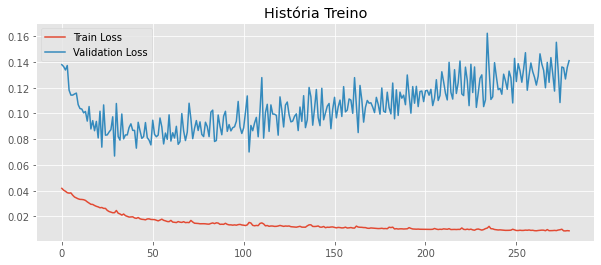
\includegraphics[width=\textwidth]{./Figuras/resultados/case1_rnn_exo_1_train.png}
        \caption{Model training RNN\_EXO\_1  in the 1st phase, RMSE = 132.94} \label{fig:case1_rnn_exo_1_train} }
        \end{figure}

     

    
        \begin{figure}[H]
          \center{
            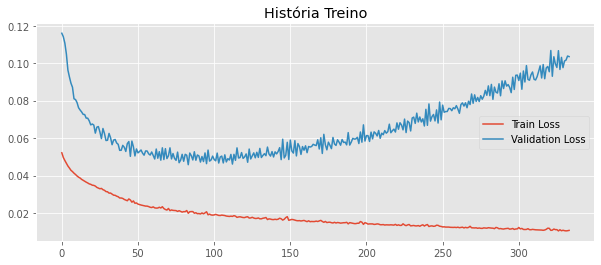
\includegraphics[width=\textwidth]{./Figuras/resultados/case2/case2_rnn_exo1_train.png}
          \caption{Model training graph RNN\_EXO\_1 in second phase, RMSE = 109.97} \label{fig:case2_rnn_exo1_train} }
        \end{figure}
    

    \subsection{Comparative test of the model in the first semester between the two phases}
    
        As this model trained in the second phase obtained the best results of the work, the metrics for the model testing within the domain of the first semester of 2019 were recalculated to make an equivalent comparison with its version trained and tested also in the first semester of 2019 in the first phase.
        
        The table \ref{table:case1_rnn_exo_1} shows that the RMSE testing model trained in the first phase performed less well than the RMSE trained in the second phase according to the table \ref{table:case2_rnn_exo_2_incase1}. The RMSE being smaller in the training of this model in the second phase brings an improvement in all other metrics compared to its training in the first phase.
        The sum of the positive prediction errors was also lower in the second phase, which impacts less on meal disposal.
        The RMSE of this model tested in the first phase and reaching RMSE = 106.208 also did better than the best model of the first phase, the RNN\_ENDO\_2 which reached RMSE = 108.06.
        
        
        
        
        \begin{table}[!ht]
            \centering
            \caption{RNN\_EXO\_1 TRAINED IN PHASE 1,TEST FIRST SEMESTER 2019}
            \label{table:case1_rnn_exo_1}
            \rowcolors{2}{gray!25}{white}
                \begin{tabular}{c|c}
                \rowcolor{gray!50}
                \hline
            \multicolumn{2}{c}{RNN\_EXO\_1 TRAINED IN PHASE 1,TEST FIRST SEMESTER 2019} \\
            \hline
            RMSE & 124.49\\
            TOTAL MEALS CONSUMED & 31962 \\
            TOTAL OF PROJECTED MEALS & 28728.816  \\
            FORECAST ERROR & -3233.1839 \\
            PERCENTAGE ERROR& -10.11\%  \\
            CORRELATION (r) & 0.41 \\ 
            P-value & 6.59e-05\\ 
            R2 & 0.16\\
            SUM OF POSITIVE ERRORS & 2709.17\\
            SUM OF NEGATIVE ERRORS & 5942.35\\
            MEDIAN ABSOLUTE ERROR & 85.59\\
            ABSOLUTE ERROR AVERAGE PERCENTAGE & 90.98\% \\ \hline \end{tabular} \end{table}
            
      
      
            \begin{table}[!ht]
            \centering
            \caption{RNN\_EXO\_1 TRAINED IN PHASE 2,TEST FIRST SEMESTER 2019}
            \label{table:case2_rnn_exo_2_incase1}
            \rowcolors{2}{gray!25}{white}
                \begin{tabular}{c|c}
                \rowcolor{gray!50}
                \hline
                \multicolumn{2}{c}{RNN\_EXO\_1 TRAINED IN PHASE 2,TEST FIRST SEMESTER 2019}\\ \hline
                RMSE & 106.2080\\
                TOTAL MEALS CONSUMED & 31962\\
                TOTAL OF PROJECTED MEALS & 32170.24\\
                FORECAST ERROR & 208.2460 \\
                PERCENTAGE ERROR & 0.6515\%  \\
                CORRELATION (r)& 0.59 \\
                P-value (p) & 1.4143e-09\\
                R2 & 0.3485\\
                SUM OF POSITIVE ERRORS & 3454.8698\\
                SUM OF NEGATIVE ERRORS & 3246.6228\\
                MEDIAN ABSOLUTE ERROR & 59.5414\\
                ABSOLUTE ERROR AVERAGE PERCENTAGE & 83.2671\% \\ \hline
            \end{tabular}
            \end{table}
                
            
            
        The scatter plot of the trained model in the first phase as shown in figure \ref{fig:case1_rnn_exo_1_test_scatter} also came out worse, farther from the upper right edge of the plot, than the scatter plot of the trained model in the second phase as shown in figure  \ref{fig:case2_rnn_exo2_test_incase1_Figura}.
        
                \begin{figure}[H]
                      \center{                    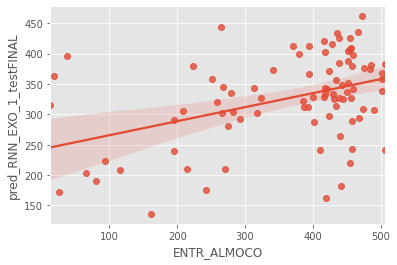
\includegraphics[width=\textwidth]{./Figuras/resultados/case1_rnn_exo_1_test_scatter.png}
                        \caption{Model test dispersion graph RNN\_EXO\_1, first phase} \label{fig:case1_rnn_exo_1_test_scatter} }
                        \end{figure}        
        


     \begin{figure}[H]
              \center{
                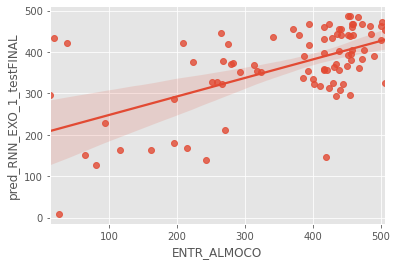
\includegraphics[width=\textwidth]{./Figuras/resultados/case2/case2_rnn_exo2_test_incase1_scatter.png}
              \caption{Test scatter plot of the first semester, RNN\_EXO\_1 trained in the second phase.} \label{fig:case2_rnn_exo2_test_incase1_Figura} }
                \end{figure}        In conclusion, when comparing the prediction graphs, the  RNN\_EXO\_1 model trained in the first phase produced worse predictions, and did not learn the weekly seasonality of consumption, as can be seen in figure  \ref{fig:case1_rnn_exo_1_test}, it is also possible to notice in table  \ref{table:case1_rnn_exo_1}, that the correlation between the predicted values and actual consumption, as well as the value  $R^2$ was lower compared to the metrics of the model trained in the second phase, and that this model trained in the second phase learned better the weekly and monthly seasonality of consumption as can be seen in the figure \ref{fig:case2_rnn_exo2_test_incase1}.
      
           
                  \begin{figure}[H]
                      \center{                    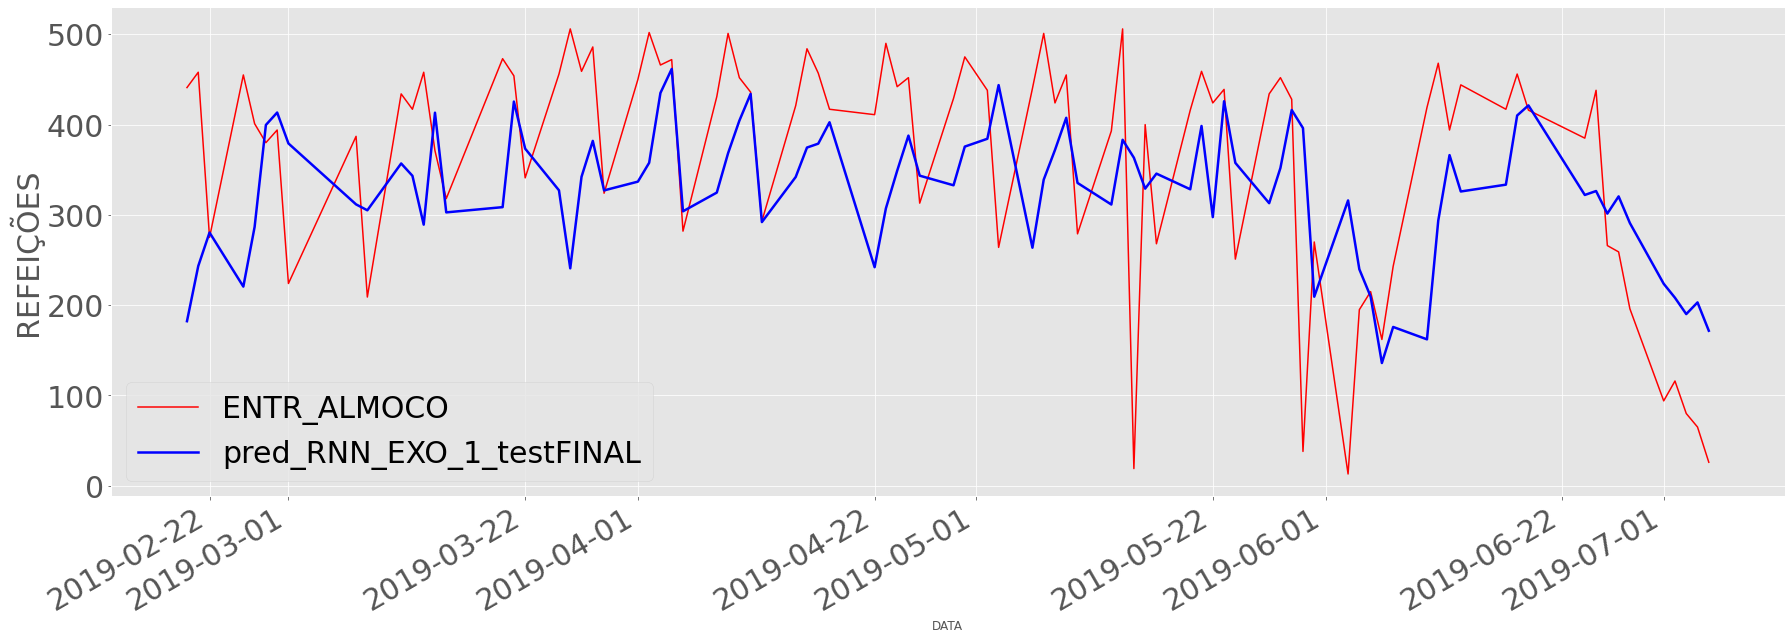
\includegraphics[width=\textwidth]{./Figuras/resultados/case1_rnn_exo_1_test.png}
                      \caption{Model Test  RNN\_EXO\_1, 1 Phase} 
                      \label{fig:case1_rnn_exo_1_test} }
                    \end{figure} 

   

            
            
      
           
           
            \begin{figure}[H]
              \center{
                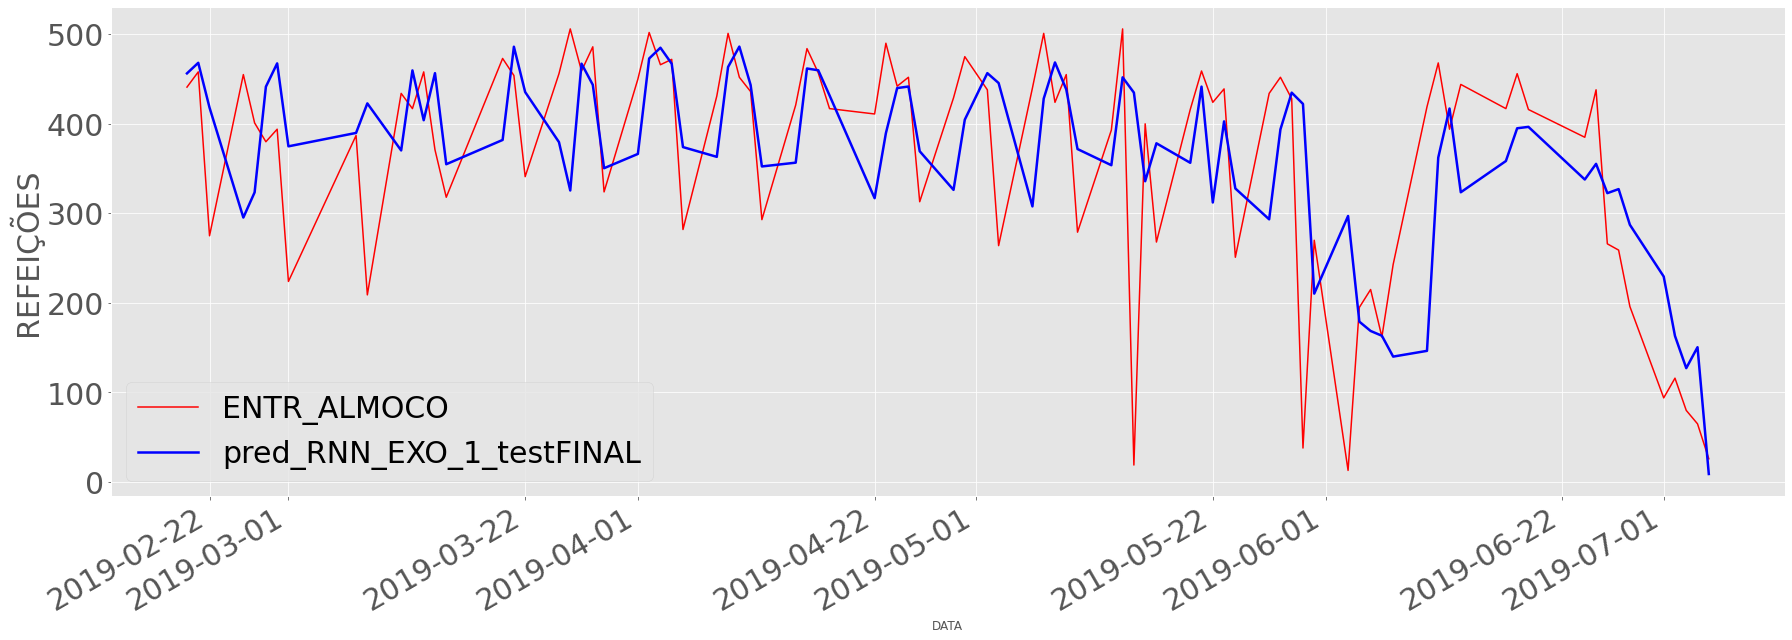
\includegraphics[width=\textwidth]{./Figuras/resultados/case2/case2_rnn_exo2_test_incase1.png}
              \caption{Test of the first semester of RNN\_EXO\_1 trained in the second phase.} \label{fig:case2_rnn_exo2_test_incase1} }
            \end{figure}
           
           
           
                
                
                
    \subsection{Final test of the  RNN\_EXO\_1 model for the ICT-Unifesp R.U predictions}
    
     The final test of RNN\_EXO\_1 produced the best results with its training in the second phase and being tested for the entire year 2019. The RMSE observed in table  \ref{table:case2_rnn_exo_2_2019} was notoriously inferior to all the models trained and tested in all the research.
     
      
        \begin{table}[!h]
            \centering
            \caption{RNN\_EXO\_1 TRAINED IN THE 2ND PHASE, TEST YEAR 2019}
            \label{table:case2_rnn_exo_2_2019}
            \rowcolors{2}{gray!25}{white}
                \begin{tabular}{c|c}
                \rowcolor{gray!50}
                \hline
                \multicolumn{2}{c}{RNN\_EXO\_1 TRAINED IN THE 2ND PHASE, TEST YEAR 2019}\\ \hline
                RMSE & 99.36\\
                TOTAL MEALS CONSUMED & 58653 \\
                TOTAL OF PROJECTED MEALS & 62048.04\\
                FORECAST ERROR & 3395.04 \\
                PERCENTAGE ERROR  & 5.78\%  \\
                CORRELATION (r)& 0.67 \\
                P-value (p) & 3.29e-25\\
                R2 & 0.45\\
                SUM OF POSITIVE ERRORS  & 8163.18\\
                SUM OF NEGATIVE ERRORS  & 4768.13\\
                MEDIAN ABSOLUTE ERROR  & 55.23\\
                ABSOLUTE ERROR AVERAGE PERCENTAGE & 83.2671\% \\ \hline
            \end{tabular}
            \end{table}

    \newpage
     The disposal of meals was obtained by the sum of the positive errors reached the value of 4768 meals.
     In the figure\ref{fig:case2_rnn_exo1_test} it is possible to notice that the model learned well the monthly and weekly seasonality of the consumption, but obtained a discrepant error for the first predicted value of the second semester, the error was justifiable because its training set contemplates only 1 year with 1 alternation of semester making impossible a better learning about this behavior.
     The scatter plot illustrated in the figure \ref{fig:case2_rnn_exo1_test_scatter} lso demonstrates a good linear regression over the predicted values of the model and the actual consumption value, approaching the identity function of an ideal forecast.
     
            %%% RNN_EXO_1
        \begin{figure}[H]
          \center{
            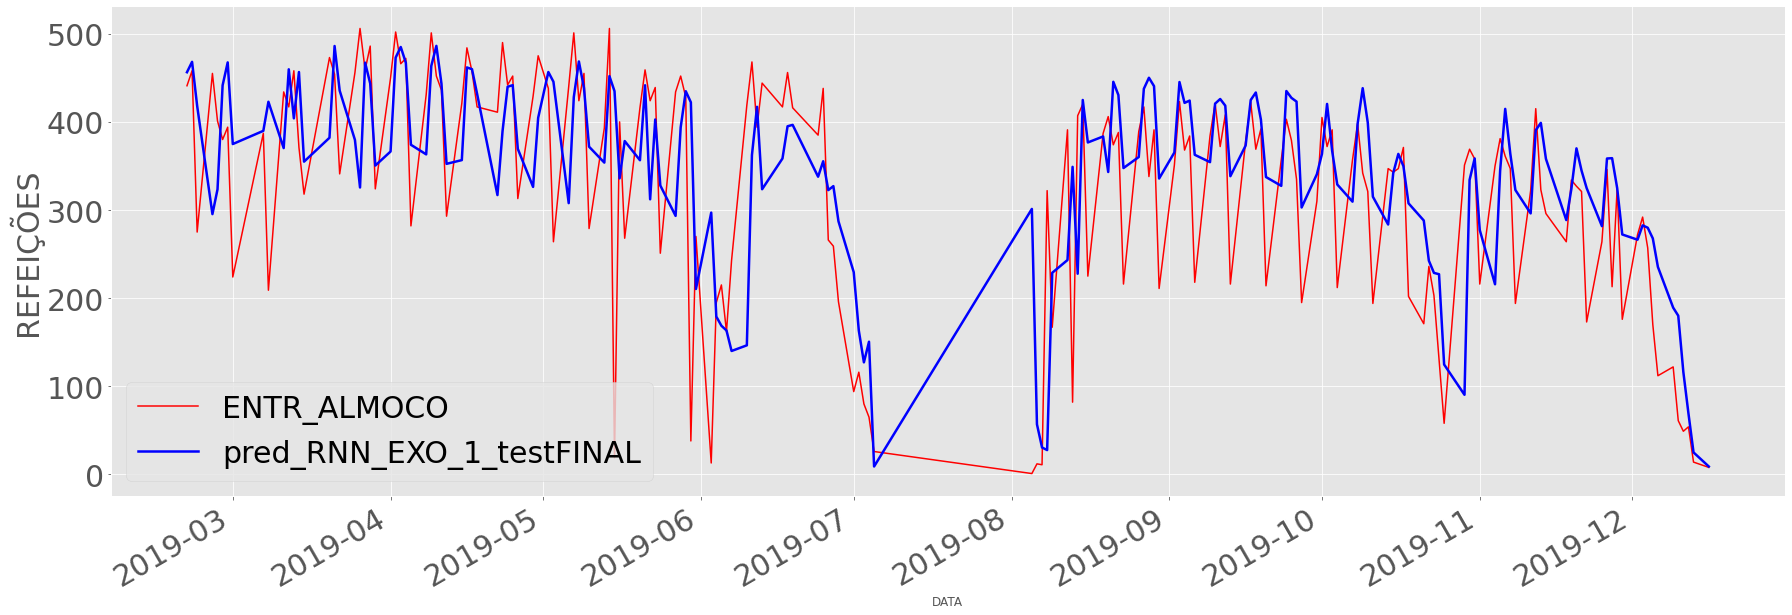
\includegraphics[width=\textwidth]{./Figuras/resultados/case2/case2_rnn_exo1_test.png}
          \caption{Final Test Graph of the Model RNN\_EXO\_1.} \label{fig:case2_rnn_exo1_test} }
        \end{figure}
       
       
        \begin{figure}[H]
          \center{
            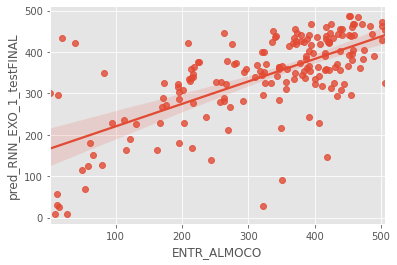
\includegraphics[width=\textwidth]{./Figuras/resultados/case2/case2_rnn_exo1_test_scatter.png}
          \caption{Model Dispersion Graph  RNN\_EXO\_1.} \label{fig:case2_rnn_exo1_test_scatter} }
        \end{figure}
        
        Results obtained by the other tested methods are available in the \ref{chapter:outros}.
       

    \chapter{Conclusão} \label{cap:conclusoes}

    Primeiramente, neste trabalho foi possível avaliar importância da metodologia de divisão do conjunto de dados em séries temporais.Visto que com um conjunto de dados de sazonalidade temporal, é notório que a ordenação dos dados na separação dos conjuntos de treino, teste e validação devem seguir uma ordem cronológica para os modelos aprenderem com o passado e realizarem predições para o futuro. O comportamento anômalo da predição identificada no capitulo de divisão do conjunto de dados da fase 1, demonstrado na figura \ref{fig:pandas_wrong_indexing}, e sua eliminação após a organização correta da série temporal, conforme a figura \ref{fig:pandas_correct_indexing}, reforça a a importancia da sequencia temporal dos dados para o correto aprendizado dos modelos testados.
    
    Com relação ao método de produção de refeições com margem de erro e análise da semana anterior foi possível observar que mesmo com a produção 30\% acima do consumo na semana anterior, no fim de cada semestre, o restaurante do ICT-Unifesp  mais do que 30\% são descartados. Este comportamento oscilatório do consumo e o acréscimo de \textit{outliers} acaba ampliando o erro dos modelos em predizer as refeições. No ano de 2019, seguindo este método, 23 mil refeições foram descartas. Neste trabalho O Modelo RNN\_EXO\_3, que apresentou o maior descarte entre todos os 12 modelos testados, obteve um valor máximo de 8914 descartes.Isso evidencia a necessidade de se implementar métodos eficientes para a produção e planejamento de refeições no restaurante universitário da Unifesp.
    
    Em relação aos ajustes empíricos da topologia dos modelos durante a etapa de validação dos primeiros modelos desenvolvidos foi possível notar a redução do RMSE ao longo do aprofundamento da rede Perceptron para treino e avaliação sob o conjunto de validação, validando a hipótese de que os modelos tem capacidade de aprendizado do problema em relação ao ajuste da topologia dos mesmos.

    Apesar do conjunto de dados conter 2 características que informam a distância em dias para o próximo registro e o registro anterior para os modelos identificarem feriados e recessos prolongados, alguns eventos no calendário, como paralisações, não são muito bem representados, indicando a necessidade de uma exploração mais aprofundada destas características que possam representar melhor este comportamento.

    Avaliando o modelo de melhor desempenho na primeira fase, com validação restrita ao primeiro semestre de 2018, os modelos endógenos se saíram melhor do que os modelos mistos. Isso pode significar que os atributos exógenos foram ruidosos durante o aprendizado aprendizado. Estes atributos são a maioria compostos de sazonalidade anual tais como as climáticas, limitadas às estações do ano. 
    O modelo RNN\_EXO\_1 da 2a fase, obteve o melhor desempenho entre todos os modelos avaliados neste trabalho, porém algumas melhorias são indicadas:
        \begin{itemize}
            \item Aumentar o conjunto de dados para o modelo se ajustar às sazonalidades semestrais e à troca de semestres. Os atributos categóricos que indicam os semestres, dia da semana, bem como os que quantificam recessos (distância registro anterior e posterior) têm potencial de agregar aprendizado nessa questão. Ainda é  necessário uma diversificação maior do conjunto de dados, dado que este modelo foi treinado apenas com 1 período de sazonalidade anual (1 ano para treino, outro ano para validação e um terceiro ano para teste).
            \item Acrescentar atributos de eventos importantes para identificar eventos e paralisações.
            \item Um atributos de cardápio tem potencial de aumentar a qualidade da predição.
            \item Um atributo representando o número de alunos matriculados em cada período de cada dia da semana tem grande potencial de aumentar a predição.
            \item Pesquisas podem ser feitas para uma melhor transformação dos dados de entrada no modelo perceptron, pois são dados discretos, enquanto os dados que entram na camada GRU são temporais (com intervalo de 5 dias).
        \end{itemize}
        
    \section{Conclusões gerais}
        
        O fenômeno mais evidente neste trabalho foi a melhoria significativa em todos os modelos de redes neurais artificiais avaliados, apenas alterando-se a organização do conjunto de dados entre a primeira e segunda fase, sem interferência em qualquer parâmetro ou hiper-parâmetro destes modelos. Assim, denota-se a necessidade de mais estudos e experimentos relacionados com organização de conjunto de dados para predições de séries temporais de consumo. As análises diversas de previsão de demanda para o tema abordado requerem extensos métodos de implementação e estruturação de dados.
        
        A aplicação de métodos de treino com retro-propagação, visto a diversidade de parâmetros no aprendizado de máquina dentro de apenas uma análise, onde pode-se montar infinitas topologias diferentes com base na estrutura dos dados coletados, tem potencial para aumentar a performance dos modelos na previsão das demandas par ao RU. 
        
        As heurísticas sobre a definição de topologia apesar de diversas, não são determinísticas, e o processo requer análise exploratória, subjetiva e empírica sobre o tema ou problema a ser abordado. Todavia, foi notória a eficiência dos modelos de aprendizado de máquina em trabalhos relacionados à restaurantes universitários. Como no caso do RU do ICT-Unifesp não há qualquer modelo atual de previsão e a falta de um modelo causa desperdício de alimentos e prejuízo ao restaurante, a abordagem desta pesquisa e sua continuação com novos métodos torna-se viável e importante para auxiliar em uma gestão assertiva dos recurso.


  % ----------------------------------------------------------
  % ELEMENTOS PÓS-TEXTUAIS
 

    %\glossary

 
  % Apêndices
 
  % ---
  % Inicia os apêndices
  % ---
  %\begin{apendicesenv}


  %\partapendices


  %\end{apendicesenv}
  % ---


  % ----------------------------------------------------------
  % Anexos
  % ----------------------------------------------------------
   % ----------------------------------------------------------
  % \chapter{Plano de atividades para o TCC II}
  % ----------------------------------------------------------

  % ---
  % Inicia os anexos
  % ---
  \begin{anexosenv}
    
  % Imprime uma página indicando o início dos anexos
  \partanexos
\nopartblankpage
    \chapter{Topologias de outros \\ modelos de redes testados}\label{cap:anexo1}
	
	\paragraph{Modelo endógeno MLP\_ENDO\_1}
        O primeiro modelo experimental MLP para obtenção das predições tem topologia definida na figura \ref{fig:case1_mlp_endo1}, denominado MLP\_ENDO\_1, este modelo tem 64 neurônios na primeira camada oculta e 32 neurônios na segunda camada oculta, e assim como todos os outros modelos, 1 neurônio na camada de saída.    
        
        \begin{figure}[h]
        	\center{                		
        	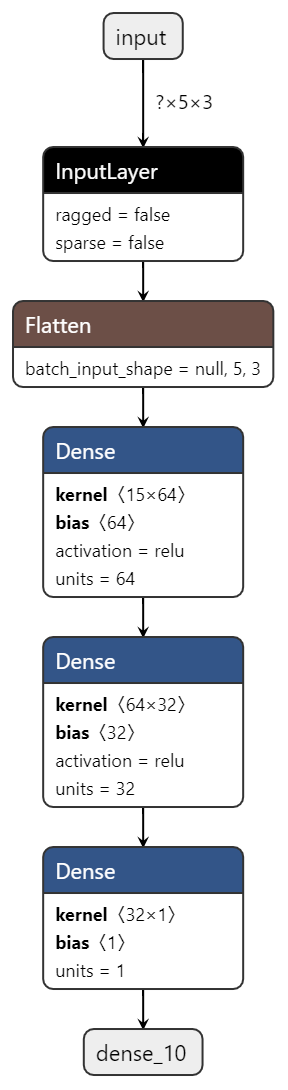
\includegraphics[width=0.4\textwidth]{./Figuras/resultados/case1_mlp_endo1.png}
        	\caption{Topologia do modelo MLP\_ENDO\_1} 
        	\label{fig:case1_mlp_endo1} 
        	}
        \end{figure}
            
    \paragraph{Modelo endógeno GRU RNN\_ENDO\_1}
        Este primeiro modelo experimental GRU foi definido com 16 unidades GRU, com topologia conceitual definida de acordo com a figura \ref{fig:gru-arch} no capítulo de fundamentação teórica \textbf{MLP\_ENDO\_1} e tem um neurônio perpcetron para emissão do sinal de saída, representado pelo bloco \textbf{Dense} na figura \ref{fig:case1_rnn_endo1}
        \begin{figure}[h]
          \center{
            \includegraphics[width=0.4\textwidth]{./Figuras/resultados/case1_rnn_endo1.png}
            \caption{Topologia do modelo RNN\_ENDO\_1} \label{fig:case1_rnn_endo1} }
        \end{figure}
        
        \paragraph{Modelo misto RNN\_EXO\_2}
         O Segundo modelo misto foi definido com o aumento da profundidade das camadas GRU e MLP do modelo anterior, conforme observado na figura \ref{fig:case1_rnn_exo_2} foram acrescentadas 1 camada GRU e 1 camada MLP (Dense).
            \begin{figure}[h]
              \center{
                \includegraphics[width=0.6\textwidth]{./Figuras/resultados/case1_rnn_exo_2.png}
              \caption{Topologia do modelo RNN\_EXO\_2}  \label{fig:case1_rnn_exo_2} }
            \end{figure}
        
        \paragraph{Modelo misto RNN\_EXO\_3}
        Para o terceiro e último modelo misto, representado na figura \ref{fig:case1_rnn_exo_3}, foi feita uma reconfiguração do modelo misto anterior, RNN\_EXO\_2, com a utilização do recurso dropout nas saídas das camadas GRU.
        \begin{figure}[h]
          \center{
          \includegraphics[width=0.5\textwidth]{./Figuras/resultados/case1_rnn_exo_3.png}
          \caption{Topologia do modelo RNN\_EXO\_3} \label{fig:case1_rnn_exo_3} 
          }
        \end{figure}
        

	\chapter{Métodos e códigos experimentais}\label{chapter:outros}

	\section{Primeira Fase Experimental}
	    \paragraph{Pré-Processamento e treino dos modelos}
	        No repositório abaixo, encontram-se os gráficos, métricas e tabelas de todos os modelos treinados na primeira fase experimental, bem como a análise exploratória detalhada de todas as variáveis e parâmetros de entrada nos modelos, e também o detalhamento do pré-processamento dos conjuntos de dados.
	        
	        Os experimentos foram realizados na plataforma Google Colab, em linguagem Python. Nenhuma configuração de ambiente é necessária para reproduzir os experimentos, bastando acessar o link para a plataforma google colab no interior do documento, através de um navegador de internet e executá-los caso seja de interesse.
	        
	        Os experimentos se encontram acessíveis em formato de documento Jupyter Notebook, com recursos de indexação e documentação com blocos de texto e imagens para uma fácil compreensão e acesso instantâneo das informações. \url{https://github.com/ddlandim/monografy-ann-demand-prediction/blob/master/case1__Experimentos_2609.ipynb}
            
	    \paragraph{Importação e aplicação de métricas dos modelos}
	        No link abaixo encontra-se uma página para a importação dos modelos contidos no repositório deste trabalho, já treinados, e encontram-se também o conjuntos de dados pré-processados para o calculo das métricas finais da primeira fase. \url{https://github.com/ddlandim/monografy-ann-demand-prediction/blob/master/case1__ModelsTests_DriverCode.ipynb}
	 
	\section{Segunda Fase Experimental}
	    \paragraph{Pré-Processamento e treino dos modelos}
	        Repositório para os gráficos, métricas e tabelas de todos os modelos treinados na segunda fase experimental. \url{https://github.com/ddlandim/monografy-ann-demand-prediction/blob/master/case2__Experimentos_2709.ipynb}
	    \paragraph{Importação e aplicação de métricas dos modelos}
	         Repositório para a importação dos modelos já treinados e conjuntos de dados já pré-processados para o calculo das métricas finais da segunda fase. \url{https://github.com/ddlandim/monografy-ann-demand-prediction/blob/master/case2__ModelsTests_DriverCode.ipynb}
	        
\section{Tabela completa das métricas de todos os modelos}
        A seguir são listadas as tabelas com todos resultados experimentais.
     
        \begin{table}[!ht]
        \caption{Previsões e erros de todos os modelos}
        \begin{adjustbox}{width=\columnwidth,center}
           \begin{tabular}{ | c | c| c | c| c | }
     \rowcolor{gray!50}
    \multirow{2}{*}{	MODELO} & TOTAL  & TOTAL  & ERRO TOTAL & ERRO TOTAL  \\ \rowcolor{gray!50}
   &                        CONSUMIDAS & PREVISTAS &  PREVISAO &  PERC PREVISAO  \\ 
    \multicolumn{5}{c}{	MODELOS ENDÓGENOS }  \\ \hline
	RNN\_ENDO\_1 1A FASE & 31962 & 30927 & -1035 & -3.2394 \\ \hline
	RNN\_ENDO\_1 2A FASE & 58653 & 60412 & 1759 & 2.9991 \\ \hline
	RNN\_ENDO\_2 1A FASE & 31962 & 31466 & -496 & -1.5530 \\ \hline
	RNN\_ENDO\_2 2A FASE & 58653 & 61855 & 3202 & 5.4594 \\ \hline
	MLP\_ENDO\_1 1A FASE & 31962 & 32370 & 408 & 1.2754 \\ \hline
	MLP\_ENDO\_1 2A FASE & 58653 & 60039 & 1385 & 2.3611 \\ \hline
	\multicolumn{5}{c}{ MODELOS EXÓGENOS }\\ \hline
	RNN\_EXO\_1 1A FASE & 31962 & 28729 & -3233. & -10.1157 \\ \hline
	RNN\_EXO\_1 2A FASE & 58653 & 62048 & 3395 & 5.7883 \\ \hline
	RNN\_EXO\_2 1A FASE & 31962 & 30823 & -1139& -3.5631 \\ \hline
	RNN\_EXO\_2 2A FASE & 58653 & 63161 & 4507 & 7.6849 \\ \hline
	RNN\_EXO\_1 1A FASE & 31962 & 29426 & -2536 & -7.9350 \\ \hline
	RNN\_EXO\_3 2A FASE & 58653 & 58348 & -305 & -0.5196 \\ \hline
	MLP\_ENDO\_1 (**) & 31962 & 31678 & -285 & -0.8901 \\ \hline
	RNN\_EXO\_1 (**) & 31962 & 32170 & 208 & 0.6515 \\ \hline
\end{tabular} \end{adjustbox}\caption*{(**) \textbf{MODELOS TREINADOS NA 2A FASE E TESTADOS NO DOMÍNIO DA 1A FASE}} \end{table} 

\begin{table}[!ht]
        \caption{Erros quantitativos de todos os modelos}
        \begin{adjustbox}{width=\columnwidth,center}
           \begin{tabular}{ | c | c| c | c| c | }
     \rowcolor{gray!50}
    \multirow{2}{*}{	MODELO} & TOTAL SOMA  & TOTAL SOMA  & ERRO ABS & ERRO ABS \\ \rowcolor{gray!50}
   &                         ERROS POSITIVOS &  ERROS NEGATIVOS &  MEDIANO&  PERC MEDIO \\ 
    \multicolumn{5}{c}{	MODELOS ENDÓGENOS }  \\ \hline
RNN\_ENDO\_1 1A FASE & -3281 & 4316 & 74.0192 & 87.4987 \\ \hline
	RNN\_ENDO\_1 2A FASE & -7709 & 5950 & 58.4248 & 107.8793 \\ \hline
	RNN\_ENDO\_2 1A FASE & -2983 & 3479 & 46.7072 & 74.9353 \\ \hline
	RNN\_ENDO\_2 2A FASE & -8335 & 5133. & 55.7799 & 101.2846 \\ \hline
	MLP\_ENDO\_1 1A FASE & -4306 & 3898 & 71.8950 & 92.5815 \\ \hline
	MLP\_ENDO\_1 2A FASE & -7097 & 5712 & 53.8804 & 98.5516 \\ \hline
	\multicolumn{5}{c}{ MODELOS EXÓGENOS }\\ \hline
RNN\_EXO\_1 1A FASE & -2709 & 5942 & 85.5910 & 90.9869 \\ \hline
	RNN\_EXO\_1 2A FASE & -8163 & 4768 & 55.2355 & 224.9068 \\ \hline
	RNN\_EXO\_2 1A FASE & -3045 & 4184 & 63.5989 & 88.2687 \\ \hline
	RNN\_EXO\_2 2A FASE & -9677 & 5170 & 64.6863 & 230.9423 \\ \hline
	RNN\_EXO\_1 1A FASE & -3418 & 5954 & 100.4442 & 98.7906 \\ \hline
	RNN\_EXO\_3 2A FASE & -8608 & 8913 & 85.1866 & 236.5670 \\ \hline
	MLP\_ENDO\_1(**) & -351 & 3797 & 65.6641 & 84.9684 \\ \hline
	RNN\_EXO\_1  (**) & -3455 & 3247 & 59.5414 & 83.2671\\ \hline
\end{tabular} \end{adjustbox}\caption*{(**) \textbf{MODELOS TREINADOS NA 2A FASE E TESTADOS NO DOMÍNIO DA 1A FASE}} \end{table} 

	    \begin{table}[!ht]
        \caption{Métricas estatísticas e de treino de todos os modelos}
        \begin{adjustbox}{width=0.8\columnwidth,center}
           \begin{tabular}{ |c | c| c | c| }
     \rowcolor{gray!50}
   {	MODELO} & r\_2 value &	std\_err & RMSE \\ \hline
     \multicolumn{4}{c}{	MODELOS ENDÓGENOS }  \\ \hline
RNN\_ENDO\_1 1A FASE&	0,2277	&0,0600&	115,5925\\ \hline
RNN\_ENDO\_1 2A FASE&	0,4034	&0,0417&	101,1817\\ \hline
RNN\_ENDO\_2 1A FASE&	0,3545	&0,0721&	108,0663\\ \hline
RNN\_ENDO\_2 2A FASE&	0,3933	&0,0474&	105,3284\\ \hline
MLP\_ENDO\_1 1A FASE&	0,2716	&0,0947&	128,0541\\ \hline
MLP\_ENDO\_1 2A FASE&	0,4354	&0,0484&	101,1515\\ \hline
	\multicolumn{4}{c}{ MODELOS EXÓGENOS }\\ \hline
RNN\_EXO\_1 1A FASE &	0,1699 &		0,0551 &		124,4907\\ \hline
RNN\_EXO\_1 2A FASE &	0,4508 &		0,0445 &		 99,3650\\ \hline
RNN\_EXO\_2 1A FASE &	0,2710 &		0,0639 &		112,9921\\ \hline
RNN\_EXO\_2 2A FASE &	0,3539 &		0,0417 &		107,8493\\ \hline
RNN\_EXO\_1 1A FASE &	0,1153 &		0,0306 &		124,6581\\ \hline
RNN\_EXO\_3 2A FASE &	0,1953 &		0,0366 &		117,0316\\ \hline
MLP\_ENDO\_1 (**)   &   0,2896 &		0,0788 &		116,6204\\ \hline
RNN\_EXO\_1  (**)   &	0,3485 &		0,0658 &		106,2080\\ \hline
\end{tabular} \end{adjustbox}\caption*{(**) \textbf{MODELOS TREINADOS NA 2A FASE E TESTADOS NO DOMÍNIO DA 1A FASE}} \end{table} 
	    
\begin{table}[!ht]
        \caption{Métricas gráficas de todos os modelos}
        \begin{adjustbox}{width=\columnwidth,center}
           \begin{tabular}{ | c | c| c | c| c |}
     \rowcolor{gray!50}
   {	MODELO} & CORRELAÇÂO &	p-value &	slope & 	intercept\\ \hline
     \multicolumn{5}{c}{	MODELOS ENDÓGENOS }  \\ \hline
RNN\_ENDO\_1 1A FASE &	0,4772&		2,5815E-06&		0,3022&		241,6487 \\ \hline
RNN\_ENDO\_1 2A FASE&	0,6351&		5,9900E-22&		0,4601&		183,6360\\ \hline
RNN\_ENDO\_2 1A FASE&	0,5954&		9,4221E-10&		0,4956&		177,5496\\ \hline
RNN\_ENDO\_2 2A FASE&	0,6271&		2,7285E-21&		0,5125&		174,6988\\ \hline
MLP\_ENDO\_1 1A FASE&	0,5212&		1,9211E-07&		0,5365&		172,9566\\ \hline
MLP\_ENDO\_1 2A FASE&	0,6599&		3,9898E-24&		0,5704&		146,0429\\ \hline
	\multicolumn{5}{c}{ MODELOS EXÓGENOS }\\ \hline
RNN\_EXO\_1 1A FASE&	0,4122&		6,5907E-05&		0,2313&		242,4375 \\ \hline
RNN\_EXO\_1 2A FASE&	0,6714&		3,2984E-25&		0,5421&		166,2111 \\ \hline
RNN\_EXO\_2 1A FASE&	0,5206&		1,9952E-07&		0,3613&		219,0125 \\ \hline
RNN\_EXO\_2 2A FASE&	0,5948&		8,3516E-19&		0,4149&		213,3027 \\ \hline
RNN\_EXO\_1 1A FASE&	0,3396&		0,00126742&		0,1025&		297,1444 \\ \hline
RNN\_EXO\_3 2A FASE&	0,4419&		4,2231E-10&		0,2424&		242,4514 \\ \hline
MLP\_ENDO\_1 (**)&		0,5382&		6,36258E-08&	0,4668&		190,4162 \\ \hline
RNN\_EXO\_1  (**)&		0,5903&		1,41433E-09&	0,4468&		203,2738 \\ \hline
\end{tabular} \end{adjustbox} \caption*{(**) \textbf{MODELOS TREINADOS NA 2A FASE E TESTADOS NO DOMÍNIO DA 1A FASE}}\end{table} 

  \end{anexosenv}
    \bookmarksetup{startatroot}%
    
    \bibliography{references}
  \end{document}